% Options for packages loaded elsewhere
%DIF LATEXDIFF DIFFERENCE FILE
%DIF DEL manuscript/v3/render.tex   Thu Mar 25 22:22:27 2021
%DIF ADD manuscript/render.tex      Mon Mar 29 13:57:11 2021
\PassOptionsToPackage{unicode}{hyperref}
\PassOptionsToPackage{hyphens}{url}
%
\documentclass[
  table,
  10pt,
  a4paper]{article}
\usepackage{lmodern}
\usepackage{amsmath}
\usepackage{ifxetex,ifluatex}
\ifnum 0\ifxetex 1\fi\ifluatex 1\fi=0 % if pdftex
  \usepackage[T1]{fontenc}
  \usepackage[utf8]{inputenc}
  \usepackage{textcomp} % provide euro and other symbols
  \usepackage{amssymb}
\else % if luatex or xetex
  \usepackage{unicode-math}
  \defaultfontfeatures{Scale=MatchLowercase}
  \defaultfontfeatures[\rmfamily]{Ligatures=TeX,Scale=1}
\fi
% Use upquote if available, for straight quotes in verbatim environments
\IfFileExists{upquote.sty}{\usepackage{upquote}}{}
\IfFileExists{microtype.sty}{% use microtype if available
  \usepackage[]{microtype}
  \UseMicrotypeSet[protrusion]{basicmath} % disable protrusion for tt fonts
}{}
\makeatletter
\@ifundefined{KOMAClassName}{% if non-KOMA class
  \IfFileExists{parskip.sty}{%
    \usepackage{parskip}
  }{% else
    \setlength{\parindent}{0pt}
    \setlength{\parskip}{6pt plus 2pt minus 1pt}}
}{% if KOMA class
  \KOMAoptions{parskip=half}}
\makeatother
\usepackage{xcolor}
\IfFileExists{xurl.sty}{\usepackage{xurl}}{} % add URL line breaks if available
\IfFileExists{bookmark.sty}{\usepackage{bookmark}}{\usepackage{hyperref}}
\hypersetup{
  pdftitle={dyngen: a multi-modal simulator for spearheading new single-cell omics analyses},
  pdfauthor={Robrecht Cannoodt*; Wouter Saelens*; Louise Deconinck; Yvan Saeys},
  hidelinks,
  pdfcreator={LaTeX via pandoc}}
\urlstyle{same} % disable monospaced font for URLs
\usepackage[margin=1in]{geometry}
%DIF 48a48-87
\usepackage{color} %DIF > 
\usepackage{fancyvrb} %DIF > 
\newcommand{\VerbBar}{|} %DIF > 
\newcommand{\VERB}{\Verb[commandchars=\\\{\}]} %DIF > 
\DefineVerbatimEnvironment{Highlighting}{Verbatim}{commandchars=\\\{\}} %DIF > 
% Add ',fontsize=\small' for more characters per line %DIF > 
\usepackage{framed} %DIF > 
\definecolor{shadecolor}{RGB}{248,248,248} %DIF > 
\newenvironment{Shaded}{\begin{snugshade}}{\end{snugshade}} %DIF > 
\newcommand{\AlertTok}[1]{\textcolor[rgb]{0.94,0.16,0.16}{#1}} %DIF > 
\newcommand{\AnnotationTok}[1]{\textcolor[rgb]{0.56,0.35,0.01}{\textbf{\textit{#1}}}} %DIF > 
\newcommand{\AttributeTok}[1]{\textcolor[rgb]{0.77,0.63,0.00}{#1}} %DIF > 
\newcommand{\BaseNTok}[1]{\textcolor[rgb]{0.00,0.00,0.81}{#1}} %DIF > 
\newcommand{\BuiltInTok}[1]{#1} %DIF > 
\newcommand{\CharTok}[1]{\textcolor[rgb]{0.31,0.60,0.02}{#1}} %DIF > 
\newcommand{\CommentTok}[1]{\textcolor[rgb]{0.56,0.35,0.01}{\textit{#1}}} %DIF > 
\newcommand{\CommentVarTok}[1]{\textcolor[rgb]{0.56,0.35,0.01}{\textbf{\textit{#1}}}} %DIF > 
\newcommand{\ConstantTok}[1]{\textcolor[rgb]{0.00,0.00,0.00}{#1}} %DIF > 
\newcommand{\ControlFlowTok}[1]{\textcolor[rgb]{0.13,0.29,0.53}{\textbf{#1}}} %DIF > 
\newcommand{\DataTypeTok}[1]{\textcolor[rgb]{0.13,0.29,0.53}{#1}} %DIF > 
\newcommand{\DecValTok}[1]{\textcolor[rgb]{0.00,0.00,0.81}{#1}} %DIF > 
\newcommand{\DocumentationTok}[1]{\textcolor[rgb]{0.56,0.35,0.01}{\textbf{\textit{#1}}}} %DIF > 
\newcommand{\ErrorTok}[1]{\textcolor[rgb]{0.64,0.00,0.00}{\textbf{#1}}} %DIF > 
\newcommand{\ExtensionTok}[1]{#1} %DIF > 
\newcommand{\FloatTok}[1]{\textcolor[rgb]{0.00,0.00,0.81}{#1}} %DIF > 
\newcommand{\FunctionTok}[1]{\textcolor[rgb]{0.00,0.00,0.00}{#1}} %DIF > 
\newcommand{\ImportTok}[1]{#1} %DIF > 
\newcommand{\InformationTok}[1]{\textcolor[rgb]{0.56,0.35,0.01}{\textbf{\textit{#1}}}} %DIF > 
\newcommand{\KeywordTok}[1]{\textcolor[rgb]{0.13,0.29,0.53}{\textbf{#1}}} %DIF > 
\newcommand{\NormalTok}[1]{#1} %DIF > 
\newcommand{\OperatorTok}[1]{\textcolor[rgb]{0.81,0.36,0.00}{\textbf{#1}}} %DIF > 
\newcommand{\OtherTok}[1]{\textcolor[rgb]{0.56,0.35,0.01}{#1}} %DIF > 
\newcommand{\PreprocessorTok}[1]{\textcolor[rgb]{0.56,0.35,0.01}{\textit{#1}}} %DIF > 
\newcommand{\RegionMarkerTok}[1]{#1} %DIF > 
\newcommand{\SpecialCharTok}[1]{\textcolor[rgb]{0.00,0.00,0.00}{#1}} %DIF > 
\newcommand{\SpecialStringTok}[1]{\textcolor[rgb]{0.31,0.60,0.02}{#1}} %DIF > 
\newcommand{\StringTok}[1]{\textcolor[rgb]{0.31,0.60,0.02}{#1}} %DIF > 
\newcommand{\VariableTok}[1]{\textcolor[rgb]{0.00,0.00,0.00}{#1}} %DIF > 
\newcommand{\VerbatimStringTok}[1]{\textcolor[rgb]{0.31,0.60,0.02}{#1}} %DIF > 
\newcommand{\WarningTok}[1]{\textcolor[rgb]{0.56,0.35,0.01}{\textbf{\textit{#1}}}} %DIF > 
%DIF -------
\usepackage{graphicx}
\makeatletter
\def\maxwidth{\ifdim\Gin@nat@width>\linewidth\linewidth\else\Gin@nat@width\fi}
\def\maxheight{\ifdim\Gin@nat@height>\textheight\textheight\else\Gin@nat@height\fi}
\makeatother
% Scale images if necessary, so that they will not overflow the page
% margins by default, and it is still possible to overwrite the defaults
% using explicit options in \includegraphics[width, height, ...]{}
\setkeys{Gin}{width=\maxwidth,height=\maxheight,keepaspectratio}
% Set default figure placement to htbp
\makeatletter
\def\fps@figure{htbp}
\makeatother
\setlength{\emergencystretch}{3em} % prevent overfull lines
\providecommand{\tightlist}{%
  \setlength{\itemsep}{0pt}\setlength{\parskip}{0pt}}
\setcounter{secnumdepth}{-\maxdimen} % remove section numbering
\usepackage{tcolorbox}
\usepackage{colortbl}
\usepackage{booktabs}
\usepackage{tabularx}
\usepackage{fontspec}
\usepackage{pifont}
\usepackage{float}
\usepackage{caption}
\captionsetup[table]{position=bottom}
\setmainfont [Path = fonts/,
  UprightFont = *-300,
  ItalicFont = *-300-Italic,
  BoldFont = *-700,
  BoldItalicFont = *-700-Italic
]{MuseoSans}

\ifluatex
  \usepackage{selnolig}  % disable illegal ligatures
\fi
\usepackage[sorting=none,url=false]{biblatex}
\addbibresource{library.bib}

\title{dyngen: a multi-modal simulator for spearheading new single-cell
omics analyses}
\author{Robrecht Cannoodt* \and Wouter Saelens* \and Louise
Deconinck \and Yvan Saeys}
\date{\DIFdelbegin \DIFdel{14 September 2020}\DIFdelend \DIFaddbegin \DIFadd{29 March 2021}\DIFaddend }
%DIF PREAMBLE EXTENSION ADDED BY LATEXDIFF
%DIF UNDERLINE PREAMBLE %DIF PREAMBLE
\RequirePackage[normalem]{ulem} %DIF PREAMBLE
\RequirePackage{color}\definecolor{RED}{rgb}{1,0,0}\definecolor{BLUE}{rgb}{0,0,1} %DIF PREAMBLE
\providecommand{\DIFaddtex}[1]{{\protect\color{blue}\uwave{#1}}} %DIF PREAMBLE
\providecommand{\DIFdeltex}[1]{{\protect\color{red}\sout{#1}}}                      %DIF PREAMBLE
%DIF SAFE PREAMBLE %DIF PREAMBLE
\providecommand{\DIFaddbegin}{} %DIF PREAMBLE
\providecommand{\DIFaddend}{} %DIF PREAMBLE
\providecommand{\DIFdelbegin}{} %DIF PREAMBLE
\providecommand{\DIFdelend}{} %DIF PREAMBLE
\providecommand{\DIFmodbegin}{} %DIF PREAMBLE
\providecommand{\DIFmodend}{} %DIF PREAMBLE
%DIF FLOATSAFE PREAMBLE %DIF PREAMBLE
\providecommand{\DIFaddFL}[1]{\DIFadd{#1}} %DIF PREAMBLE
\providecommand{\DIFdelFL}[1]{\DIFdel{#1}} %DIF PREAMBLE
\providecommand{\DIFaddbeginFL}{} %DIF PREAMBLE
\providecommand{\DIFaddendFL}{} %DIF PREAMBLE
\providecommand{\DIFdelbeginFL}{} %DIF PREAMBLE
\providecommand{\DIFdelendFL}{} %DIF PREAMBLE
%DIF HYPERREF PREAMBLE %DIF PREAMBLE
\providecommand{\DIFadd}[1]{\texorpdfstring{\DIFaddtex{#1}}{#1}} %DIF PREAMBLE
\providecommand{\DIFdel}[1]{\texorpdfstring{\DIFdeltex{#1}}{}} %DIF PREAMBLE
\newcommand{\DIFscaledelfig}{0.5}
%DIF HIGHLIGHTGRAPHICS PREAMBLE %DIF PREAMBLE
\RequirePackage{settobox} %DIF PREAMBLE
\RequirePackage{letltxmacro} %DIF PREAMBLE
\newsavebox{\DIFdelgraphicsbox} %DIF PREAMBLE
\newlength{\DIFdelgraphicswidth} %DIF PREAMBLE
\newlength{\DIFdelgraphicsheight} %DIF PREAMBLE
% store original definition of \includegraphics %DIF PREAMBLE
\LetLtxMacro{\DIFOincludegraphics}{\includegraphics} %DIF PREAMBLE
\newcommand{\DIFaddincludegraphics}[2][]{{\color{blue}\fbox{\DIFOincludegraphics[#1]{#2}}}} %DIF PREAMBLE
\newcommand{\DIFdelincludegraphics}[2][]{% %DIF PREAMBLE
\sbox{\DIFdelgraphicsbox}{\DIFOincludegraphics[#1]{#2}}% %DIF PREAMBLE
\settoboxwidth{\DIFdelgraphicswidth}{\DIFdelgraphicsbox} %DIF PREAMBLE
\settoboxtotalheight{\DIFdelgraphicsheight}{\DIFdelgraphicsbox} %DIF PREAMBLE
\scalebox{\DIFscaledelfig}{% %DIF PREAMBLE
\parbox[b]{\DIFdelgraphicswidth}{\usebox{\DIFdelgraphicsbox}\\[-\baselineskip] \rule{\DIFdelgraphicswidth}{0em}}\llap{\resizebox{\DIFdelgraphicswidth}{\DIFdelgraphicsheight}{% %DIF PREAMBLE
\setlength{\unitlength}{\DIFdelgraphicswidth}% %DIF PREAMBLE
\begin{picture}(1,1)% %DIF PREAMBLE
\thicklines\linethickness{2pt} %DIF PREAMBLE
{\color[rgb]{1,0,0}\put(0,0){\framebox(1,1){}}}% %DIF PREAMBLE
{\color[rgb]{1,0,0}\put(0,0){\line( 1,1){1}}}% %DIF PREAMBLE
{\color[rgb]{1,0,0}\put(0,1){\line(1,-1){1}}}% %DIF PREAMBLE
\end{picture}% %DIF PREAMBLE
}\hspace*{3pt}}} %DIF PREAMBLE
} %DIF PREAMBLE
\LetLtxMacro{\DIFOaddbegin}{\DIFaddbegin} %DIF PREAMBLE
\LetLtxMacro{\DIFOaddend}{\DIFaddend} %DIF PREAMBLE
\LetLtxMacro{\DIFOdelbegin}{\DIFdelbegin} %DIF PREAMBLE
\LetLtxMacro{\DIFOdelend}{\DIFdelend} %DIF PREAMBLE
\DeclareRobustCommand{\DIFaddbegin}{\DIFOaddbegin \let\includegraphics\DIFaddincludegraphics} %DIF PREAMBLE
\DeclareRobustCommand{\DIFaddend}{\DIFOaddend \let\includegraphics\DIFOincludegraphics} %DIF PREAMBLE
\DeclareRobustCommand{\DIFdelbegin}{\DIFOdelbegin \let\includegraphics\DIFdelincludegraphics} %DIF PREAMBLE
\DeclareRobustCommand{\DIFdelend}{\DIFOaddend \let\includegraphics\DIFOincludegraphics} %DIF PREAMBLE
\LetLtxMacro{\DIFOaddbeginFL}{\DIFaddbeginFL} %DIF PREAMBLE
\LetLtxMacro{\DIFOaddendFL}{\DIFaddendFL} %DIF PREAMBLE
\LetLtxMacro{\DIFOdelbeginFL}{\DIFdelbeginFL} %DIF PREAMBLE
\LetLtxMacro{\DIFOdelendFL}{\DIFdelendFL} %DIF PREAMBLE
\DeclareRobustCommand{\DIFaddbeginFL}{\DIFOaddbeginFL \let\includegraphics\DIFaddincludegraphics} %DIF PREAMBLE
\DeclareRobustCommand{\DIFaddendFL}{\DIFOaddendFL \let\includegraphics\DIFOincludegraphics} %DIF PREAMBLE
\DeclareRobustCommand{\DIFdelbeginFL}{\DIFOdelbeginFL \let\includegraphics\DIFdelincludegraphics} %DIF PREAMBLE
\DeclareRobustCommand{\DIFdelendFL}{\DIFOaddendFL \let\includegraphics\DIFOincludegraphics} %DIF PREAMBLE
%DIF LISTINGS PREAMBLE %DIF PREAMBLE
\RequirePackage{listings} %DIF PREAMBLE
\RequirePackage{color} %DIF PREAMBLE
\lstdefinelanguage{DIFcode}{ %DIF PREAMBLE
%DIF DIFCODE_UNDERLINE %DIF PREAMBLE
  moredelim=[il][\color{red}\sout]{\%DIF\ <\ }, %DIF PREAMBLE
  moredelim=[il][\color{blue}\uwave]{\%DIF\ >\ } %DIF PREAMBLE
} %DIF PREAMBLE
\lstdefinestyle{DIFverbatimstyle}{ %DIF PREAMBLE
	language=DIFcode, %DIF PREAMBLE
	basicstyle=\ttfamily, %DIF PREAMBLE
	columns=fullflexible, %DIF PREAMBLE
	keepspaces=true %DIF PREAMBLE
} %DIF PREAMBLE
\lstnewenvironment{DIFverbatim}{\lstset{style=DIFverbatimstyle}}{} %DIF PREAMBLE
\lstnewenvironment{DIFverbatim*}{\lstset{style=DIFverbatimstyle,showspaces=true}}{} %DIF PREAMBLE
%DIF END PREAMBLE EXTENSION ADDED BY LATEXDIFF

\begin{document}
\maketitle

\hypertarget{abstract}{%
\section{Abstract}\label{abstract}}

We present dyngen, a novel, multi-modal simulation engine for studying
dynamic cellular processes at single-cell resolution. dyngen is more
flexible than current single-cell simulation engines, and allows better
method development and benchmarking, thereby stimulating development and
testing of novel computational methods. We demonstrate its potential for
spearheading novel computational methods on three novel applications:
aligning cell developmental trajectories, \DIFdelbegin \DIFdel{single-cell }\DIFdelend \DIFaddbegin \DIFadd{cell-specific }\DIFaddend regulatory
network inference and estimation of RNA velocity.

\hypertarget{main-text}{%
\section{Main text}\label{main-text}}

Single-cell simulation engines are becoming increasingly important for
testing and benchmarking computational methods, a pressing need in the
widely expanding field of single-cell biology. Complementary to real
biological data, synthetic data provides a valuable alternative where
the actual ground truth is completely known and thus can be compared to,
in order to make quantitative evaluations of computational methods that
aim to reconstruct this ground truth
\autocite{zappia_splattersimulationsinglecell_2017}. In addition,
simulation engines are more flexible when it comes to stress-testing
computational methods, for example by varying the parameters of the
simulation, such as the amount of noise, samples, and cells measured,
allowing benchmarking of methods over a wide range of possible
scenarios. In this way, they can even guide the design of real
biological experiments, finding out the best conditions to be used as
input for subsequent computational pipelines.
\DIFaddbegin 

\DIFaddend Another, more experimental use of simulation engines is their important
role in spearheading the development of novel computational methods,
possibly even before real data is available. In this way, simulation
engines can be used to assess the value of novel experimental protocols
or treatments. Simulation engines are also increasingly important when
it comes to finding alternatives to animal models, for example for drug
testing and precision medicine. In such scenarios, cellular simulations
can act as digital twins, offering unlimited experimentation \emph{in
silico} \autocite{bjornsson_digitaltwinspersonalize_2019}.

\DIFdelbegin \DIFdel{Here, we introduce dyngen, a novel multi-modal simulator of dynamic
biological processes at }\DIFdelend \DIFaddbegin \DIFadd{Simulating realistic data requires that the underlying biology is
recapitulated as best as possible, and in the case of transcriptomics
data this typically involves modelling the underlying gene regulatory
networks. Simulators of ``bulk'' microarray or RNA-sequencing profiles
simulate biological processes (e.g.~transcription, translation) by
translating a database of known regulatory interactions into a set of
ordinary differential equations (ODE)
}\autocite{roy_systemgeneratingtranscription_2008,hache_gengesystematicgeneration_2009,schaffter_genenetweaversilicobenchmark_2011,vandenbulcke_syntrengeneratorsynthetic_2006}\DIFadd{.
These methods have been instrumental in performing benchmarking studies
}\autocite{prill_rigorousassessmentsystems_2010,marbach_revealingstrengthsweaknesses_2010,marbach_wisdomcrowdsrobust_2012}\DIFadd{.
However, the advent of }\DIFaddend single-cell \DIFdelbegin \DIFdel{resolution
(Figure~\ref{fig:overview}).dyngen uses Gillespie's stochastic
simulation algorithm }%DIFDELCMD < \autocite{gillespie_exactstochasticsimulation_1977}
%DIFDELCMD < %%%
\DIFdel{to simulate gene regulation, splicing, and translationat a single-molecule level.
Other generators of scRNA-seq data }\DIFdelend \DIFaddbegin \DIFadd{omics introduced several new types of
analyses }\DIFaddend (e.g.~\DIFdelbegin \DIFdel{splatter
}\DIFdelend \DIFaddbegin \DIFadd{trajectory inference, RNA velocity, cell-specific network
inference) which exploit the higher resolution of single-cell versus
bulk omics }\autocite{luecken_currentbestpractices_2019}\DIFadd{. In addition,
the data characteristics of single-cell omics are vastly different from
bulk omics, typically having much lower library sizes and a higher
dropout rate, but also a high number of profiles
}\autocite{vallejos_normalizingsinglecellrna_2017}\DIFadd{. The low library
sizes, in particular, are problematic as ODEs are ill-suited for
performing low-molecule simulations
}\autocite{gillespie_exactstochasticsimulation_1977}\DIFadd{. This necessitates
the development of new single-cell simulators.
}

\DIFadd{To this end, single-cell omics simulators emulate the technical
procedures from single-cell omics protocols. Simulators such as Splatter
}\DIFaddend \autocite{zappia_splattersimulationsinglecell_2017}, powsimR
\autocite{vieth_powsimrpoweranalysis_2017}, PROSSTT
\autocite{papadopoulos_prossttprobabilisticsimulation_2019} and SymSim
\autocite{zhang_simulatingmultiplefaceted_2019}) have already been
\DIFdelbegin \DIFdel{used
extensively to explore the strengths and weaknesses of computational
tools, both by method developers
}%DIFDELCMD < \autocite{street_slingshotcelllineage_2018,parra_reconstructingcomplexlineage_2019,lummertzdarocha_reconstructioncomplexsinglecell_2018,lin_scclassifyhierarchicalclassification_2019}
%DIFDELCMD < %%%
\DIFdel{and independent benchmarkers
}\DIFdelend \DIFaddbegin \DIFadd{widely used to compare single-cell methods
}\autocite{street_slingshotcelllineage_2018,parra_reconstructingcomplexlineage_2019,lummertzdarocha_reconstructioncomplexsinglecell_2018,lin_scclassifysamplesize_2020}
\DIFadd{and perform independent benchmarks
}\DIFaddend \autocite{duo_systematicperformanceevaluation_2018,saelens_comparisonsinglecelltrajectory_2019,soneson_biasrobustnessscalability_2018}.
However, \DIFdelbegin \DIFdel{a limitation of these existing simulators is that they would
require significant methodological alterations to add }\DIFdelend \DIFaddbegin \DIFadd{by focusing more on simulating the single-cell omics protocol
(e.g.~RNA capture, amplification, sequencing) and less on the underlying
biology (e.g.~transcription, splicing, translation), their applicability
and reusability is limited towards the specific application for which
they were designed (e.g.~benchmarking clustering or differential
expression methods), and extending these tools to include }\DIFaddend additional
modalities or experimental conditions \DIFdelbegin \DIFdel{(Table~\ref{tab:comparison}).
}\DIFdelend \DIFaddbegin \DIFadd{is challenging.
}\DIFaddend 

\DIFdelbegin %DIFDELCMD < \begin{figure}[t!]
%DIFDELCMD <     \centering
%DIFDELCMD <     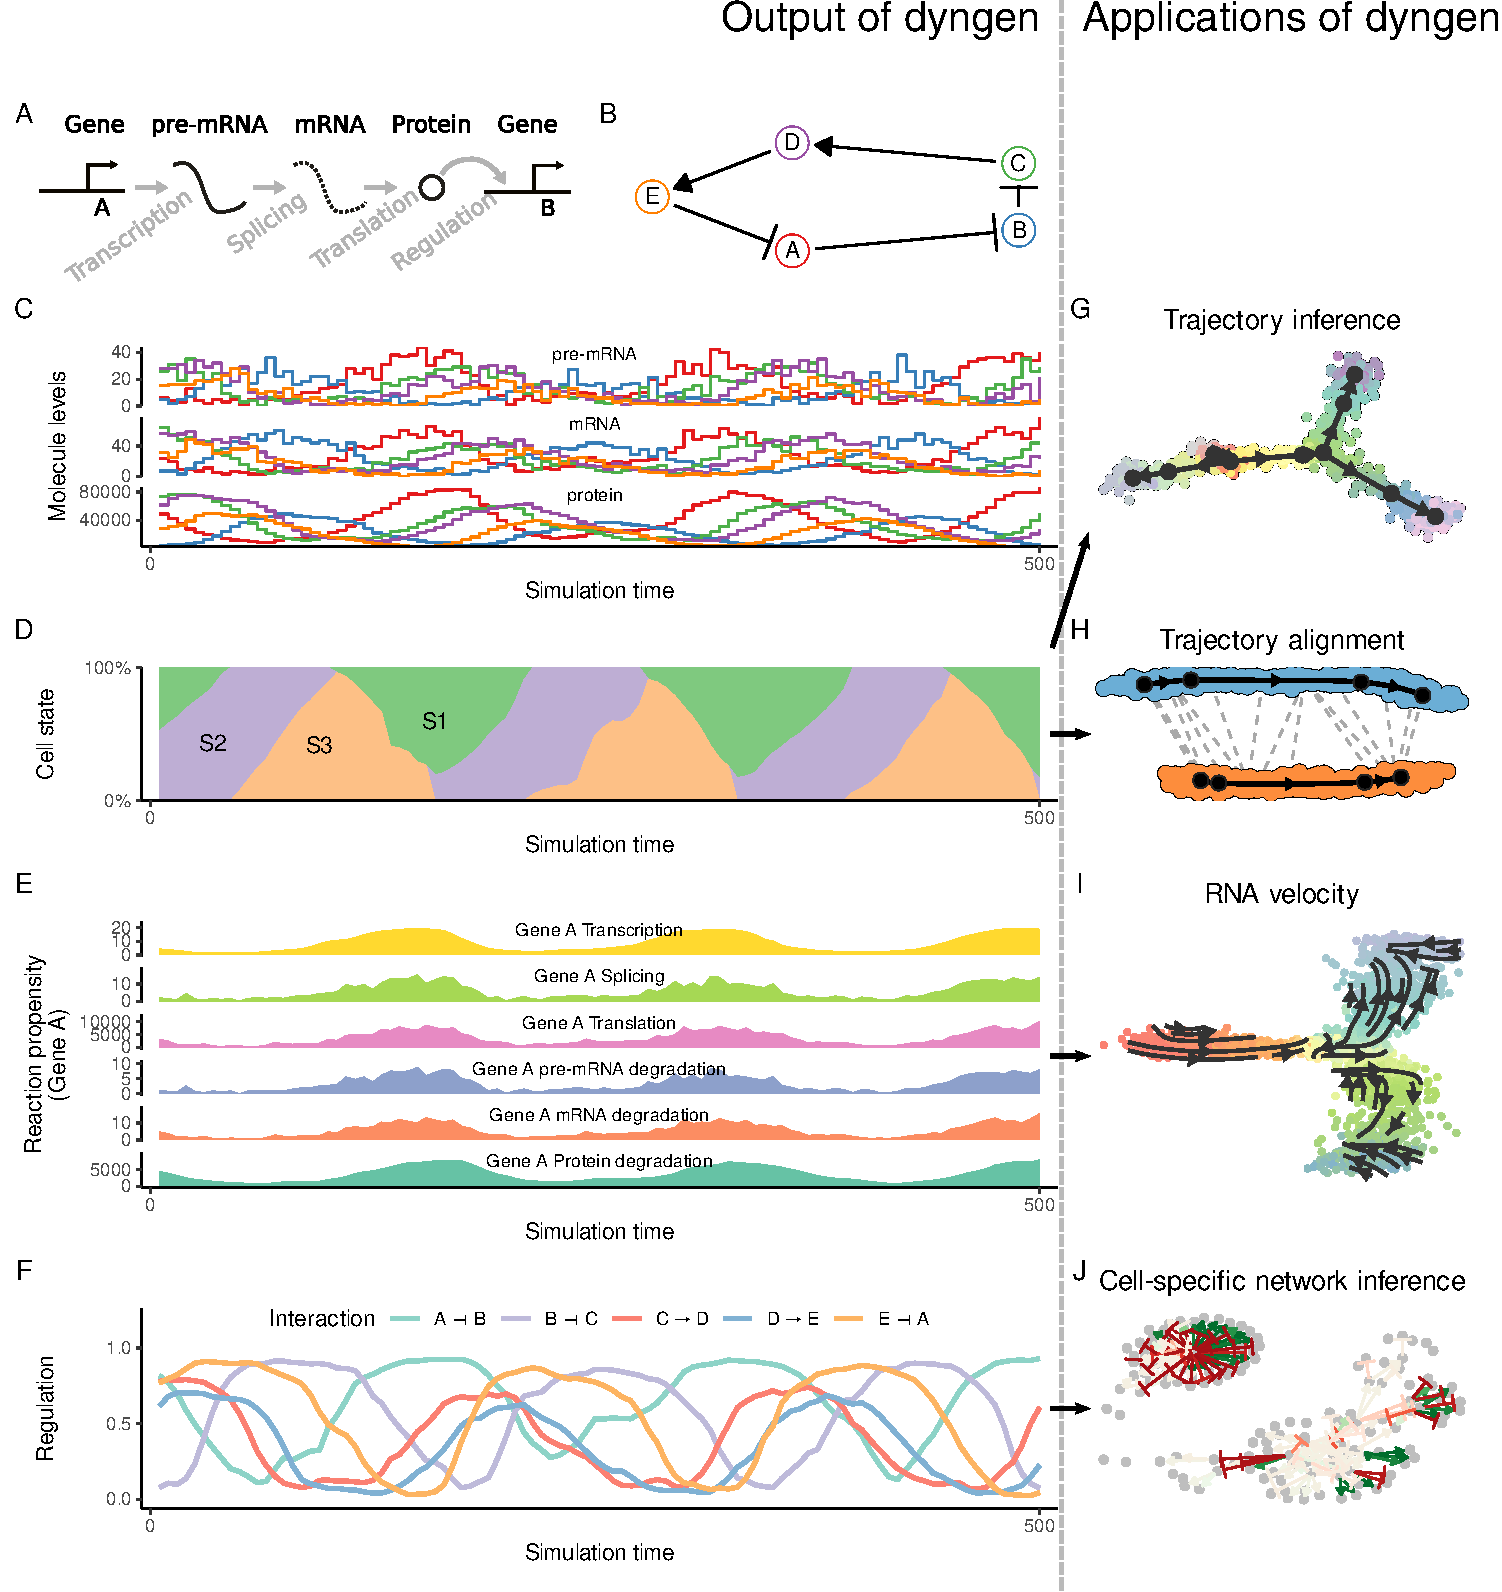
\includegraphics[width=\linewidth]{result_files/summary/figure_1_edited.pdf}
%DIFDELCMD <     %%%
%DIFDELCMD < \caption{%
{%DIFAUXCMD
\textbf{\DIFdelFL{Showcase of dyngen functionality.}}
      %DIFAUXCMD
\textbf{\DIFdelFL{A:}} %DIFAUXCMD
\DIFdelFL{Changes in abundance levels are driven strictly by gene regulatory reactions.
      }\textbf{\DIFdelFL{B:}} %DIFAUXCMD
\DIFdelFL{The input Gene Regulatory Network (GRN) is defined such that it models a dynamic process of interest.
      }\textbf{\DIFdelFL{C:}} %DIFAUXCMD
\DIFdelFL{The reactions define how abundance levels of molecules change at any particular time point.
      }\textbf{\DIFdelFL{D:}} %DIFAUXCMD
\DIFdelFL{Firing many reactions can significantly alter the cellular state over time.
      }\textbf{\DIFdelFL{E:}} %DIFAUXCMD
\DIFdelFL{dyngen keeps track of the likelihood of a reaction firing during small intervals of time, called the propensity, as well as the actual number of firings.
      }\textbf{\DIFdelFL{F:}} %DIFAUXCMD
\DIFdelFL{Similarly, dyngen can also keep track of the regulatory activity of every interaction.
      }\textbf{\DIFdelFL{G:}} %DIFAUXCMD
\DIFdelFL{A benchmark of trajectory inference methods has already been performed using the cell state ground-truth.
      }\textbf{\DIFdelFL{H:}} %DIFAUXCMD
\DIFdelFL{The cell state ground-truth enables evaluating trajectory alignment methods \mbox{%DIFAUXCMD
\cite{saelens_comparisonsinglecelltrajectory_2019}}\hspace{0pt}%DIFAUXCMD
.
      }\textbf{\DIFdelFL{I:}} %DIFAUXCMD
\DIFdelFL{The reaction propensity ground-truth enables evaluating RNA velocity methods.
      }\textbf{\DIFdelFL{J:}} %DIFAUXCMD
\DIFdelFL{The cellwise regulatory network ground-truth enables evaluating cell-specific gene regulatory network inference methods.
    }}
    %DIFAUXCMD
%DIFDELCMD < \label{fig:overview}
%DIFDELCMD < \end{figure}
%DIFDELCMD < %%%
\DIFdelend \DIFaddbegin \DIFadd{We introduce dyngen, a method for simulating cellular dynamics at a
single-cell, single-transcript resolution (Figure~\ref{fig:overview}).
This problem is tackled in three fully-configurable main steps. First,
biological processes are mimicked by translating a gene regulatory
network into a set of reactions (regulation, transcription, splicing,
translation). Second, individual cells are simulated using Gillespie's
stochastic simulation algorithm
}\autocite{gillespie_exactstochasticsimulation_1977}\DIFadd{, which is designed
to work well in low-molecule simulations. Finally, real reference
datasets are used to emulate single-cell omics profiling protocols.
}\DIFaddend 

\DIFdelbegin \DIFdel{dyngen was designed
to include all of these functionalities and more by
design. Its methodology allows tracking }\DIFdelend \DIFaddbegin \DIFadd{Throughout a simulation, dyngen tracks }\DIFaddend many layers of information\DIFdelbegin \DIFdel{throughout the simulation}\DIFdelend ,
including the abundance of any molecule in the cell, the progression of
the cell along a dynamic process, and the activation strength of
individual regulatory interactions. \DIFaddbegin \DIFadd{In addition, }\DIFaddend dyngen can simulate a
large variety of dynamic processes (e.g.~cyclic, branching,
disconnected) as well as a broad range of experimental conditions
(e.g.~batch effects and time-series, perturbation and \DIFaddbegin \DIFadd{single-cell
}\DIFaddend knockdown experiments). \DIFdelbegin \DIFdel{The fine-grained controls over simulation parameters allow
dyngen to be applicable to a broad range of use-cases to simulate
dynamic biological processes. The original design of dyngen was
motivated by the plethora of methods available for }\DIFdelend \DIFaddbegin \DIFadd{For these reasons, dyngen can cater to a wide
range of benchmarking applications, including }\DIFaddend trajectory inference,
\DIFdelbegin \DIFdel{where dyngen allowed the first large-scale benchmarking of such methods
}%DIFDELCMD < \autocite{saelens_comparisonsinglecelltrajectory_2019,vandenberge_trajectorybaseddifferentialexpression_2020}%%%
\DIFdelend \DIFaddbegin \DIFadd{trajectory alignment, and trajectory differential expression
(Table~\ref{tab:comparison})}\DIFaddend .

\DIFdelbegin \DIFdel{Here, we highlight the novel functionality of dyngen}\DIFdelend \DIFaddbegin \begin{figure}[t!]
    \centering
    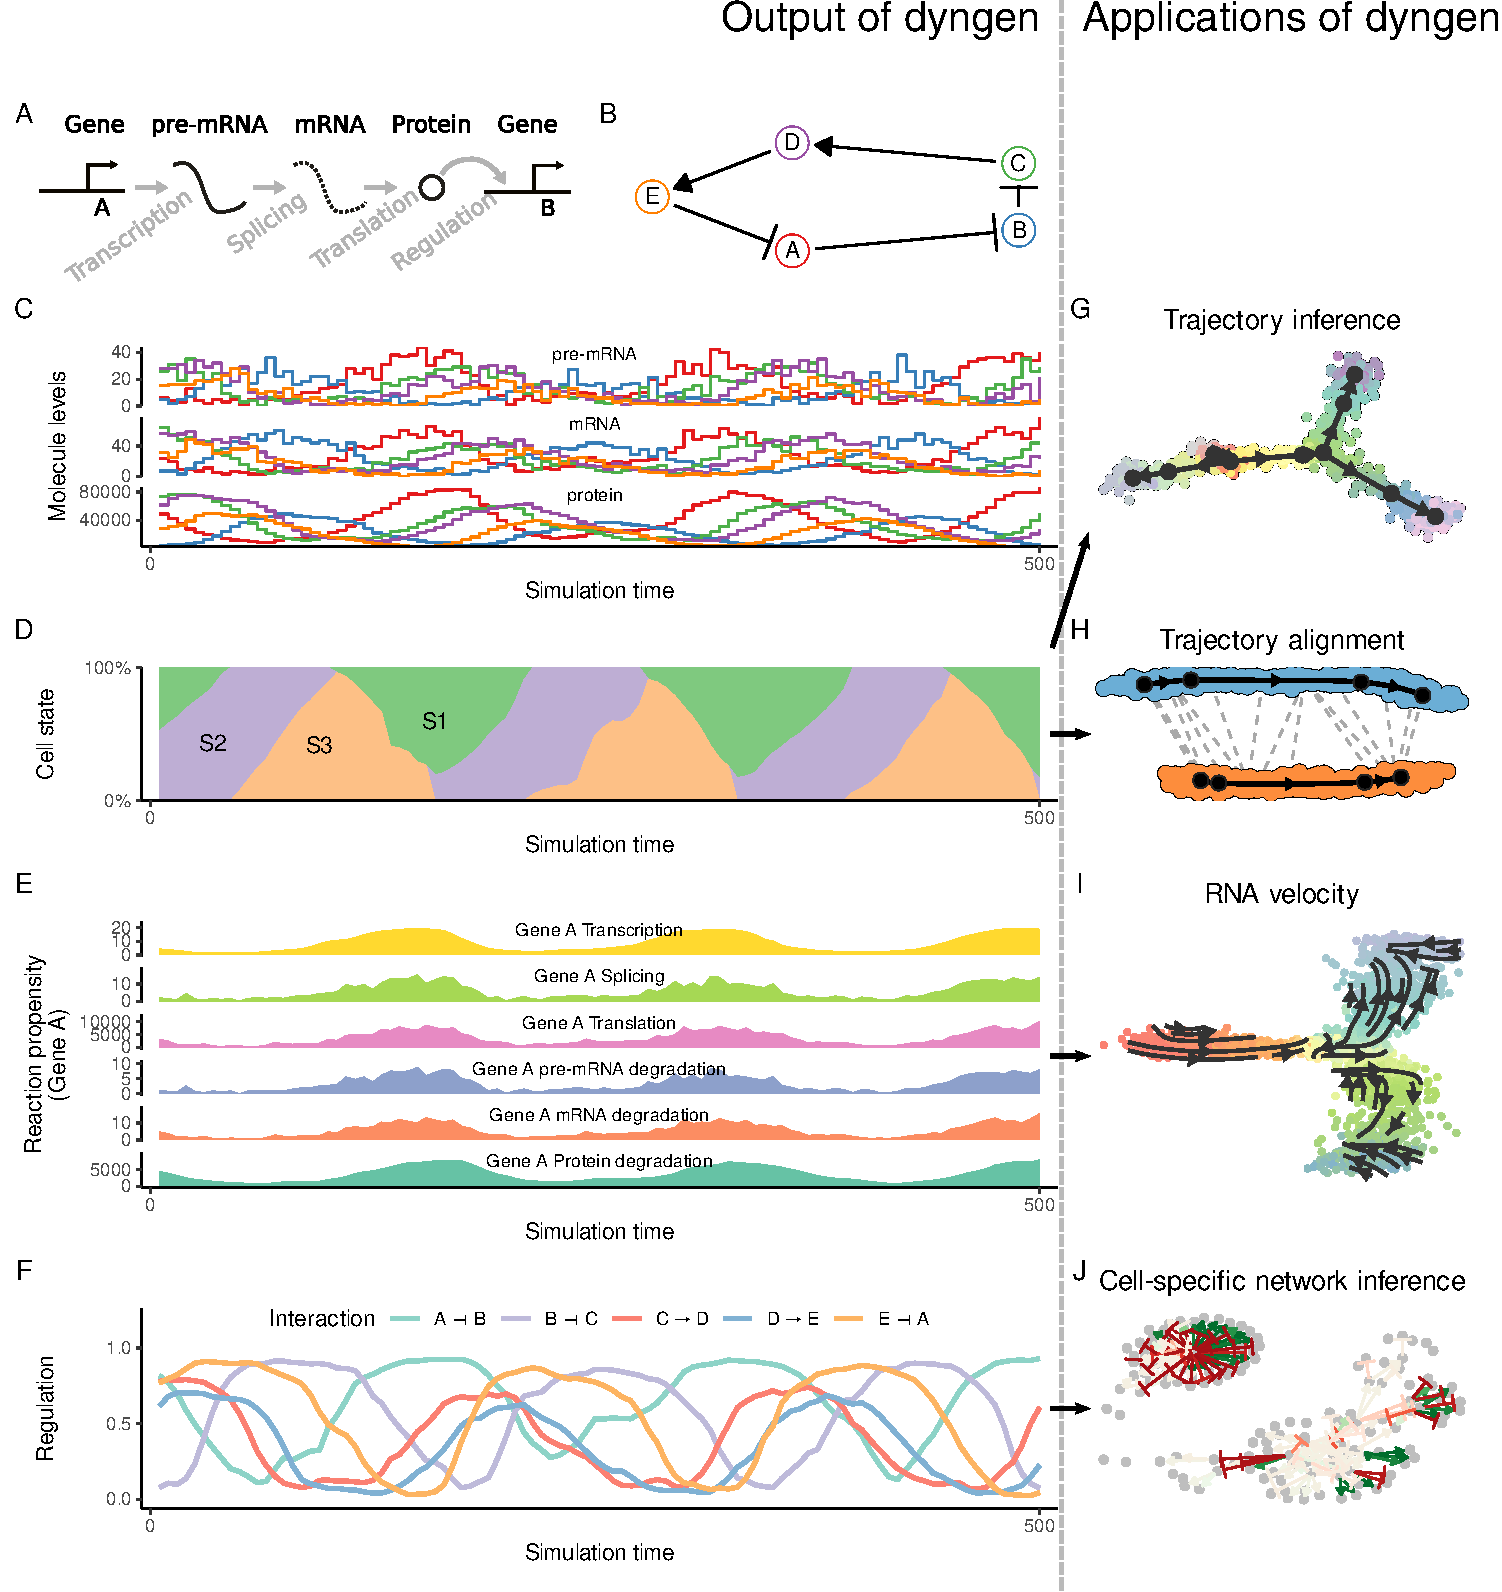
\includegraphics[width=\linewidth]{result_files/summary/figure_1_edited.pdf}
    \caption{
      \textbf{\DIFaddFL{Showcase of dyngen functionality.}}
      \textbf{\DIFaddFL{A:}} \DIFaddFL{Changes in abundance levels are driven strictly by gene regulatory reactions.
      }\textbf{\DIFaddFL{B:}} \DIFaddFL{The input Gene Regulatory Network (GRN) is defined such that it models a dynamic process of interest.
      }\textbf{\DIFaddFL{C:}} \DIFaddFL{The reactions define how abundance levels of molecules change at any particular time point.
      }\textbf{\DIFaddFL{D:}} \DIFaddFL{Firing many reactions can significantly alter the cellular state over time.
      }\textbf{\DIFaddFL{E:}} \DIFaddFL{dyngen keeps track of the likelihood of a reaction firing during small intervals of time, called the propensity, as well as the actual number of firings.
      }\textbf{\DIFaddFL{F:}} \DIFaddFL{Similarly, dyngen can also keep track of the regulatory activity of every interaction.
      }\textbf{\DIFaddFL{G:}} \DIFaddFL{A benchmark of trajectory inference methods has already been performed using the cell state ground-truth \mbox{%DIFAUXCMD
\cite{saelens_comparisonsinglecelltrajectory_2019}}\hspace{0pt}%DIFAUXCMD
.
      }\textbf{\DIFaddFL{H:}} \DIFaddFL{The cell state ground-truth enables evaluating trajectory alignment methods.
      }\textbf{\DIFaddFL{I:}} \DIFaddFL{The reaction propensity ground-truth enables evaluating RNA velocity methods.
      }\textbf{\DIFaddFL{J:}} \DIFaddFL{The cellwise regulatory network ground-truth enables evaluating cell-specific gene regulatory network inference methods.
    }}
    \label{fig:overview}
\end{figure}

\DIFadd{We demonstrate dyngen's broad applicability }\DIFaddend by evaluating three novel
types of computational approaches for which no simulation engines exist
yet: \DIFdelbegin \DIFdel{single-cell }\DIFdelend \DIFaddbegin \DIFadd{cell-specific }\DIFaddend network inference, trajectory alignment and RNA
velocity (Figure~\ref{fig:applications}). We emphasize that our main aim
here is to illustrate the potential of dyngen for these evaluations,
rather than performing large-scale benchmarking, which would require
assessing many more quantitative and qualitative aspects of each method
\autocite{weber_essentialguidelinescomputational_2019}.

\begin{figure}[t!]
    \centering
    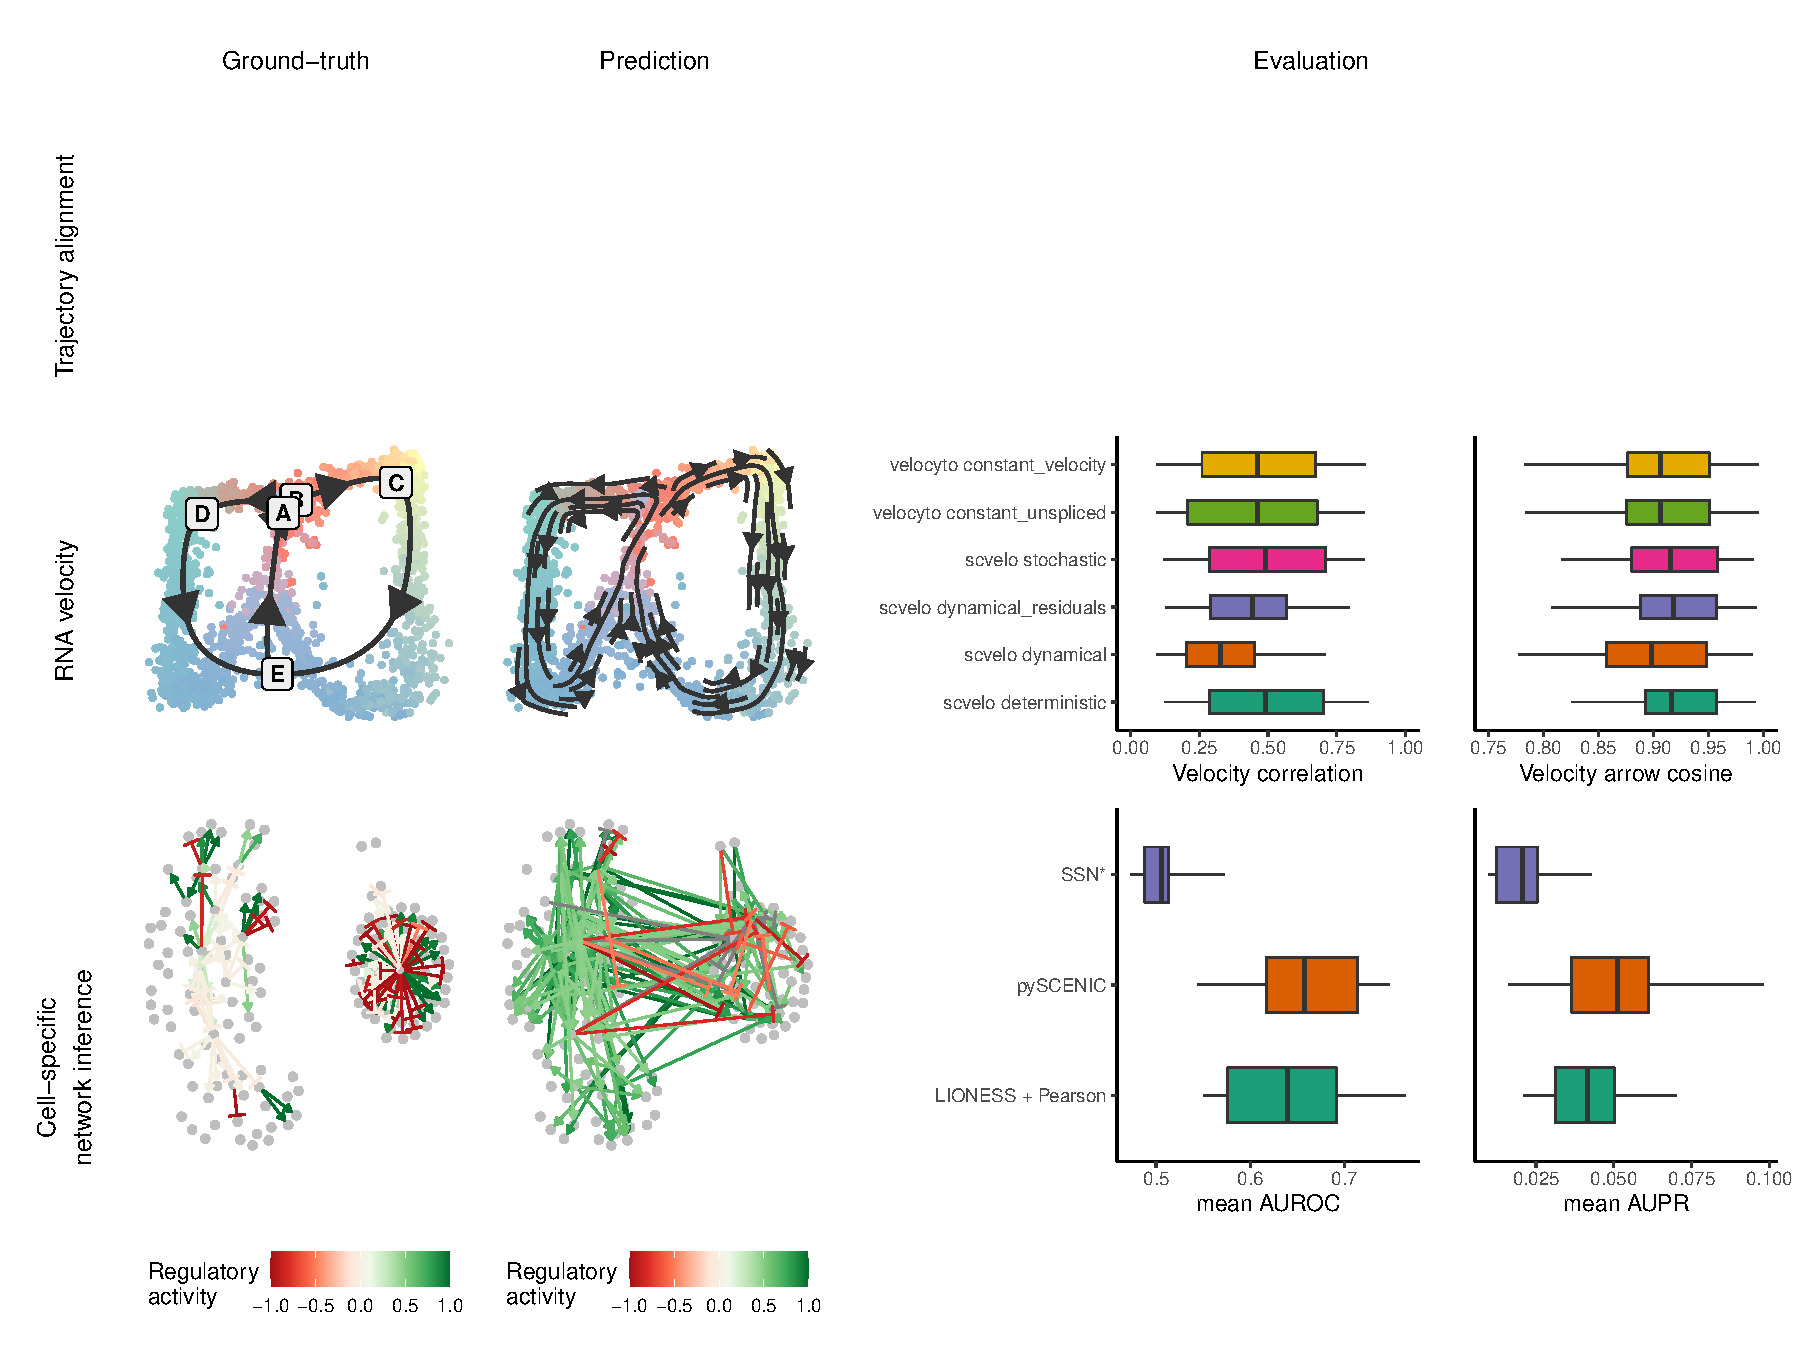
\includegraphics[width=\linewidth]{result_files/summary/figure_2.pdf}
    \caption{
      \textbf{dyngen provides ground-truth data for a variety of applications (left), which can be used to quantitatively evaluate methods (right).}
      \textbf{A:} Trajectory alignment aligns two trajectories between samples. \DIFdelbeginFL \DIFdelFL{dyngen can simulate different scenarios in which alignment is necessary, such as a premature stop as shown here. }\DIFdelendFL We \DIFdelbeginFL \DIFdelFL{compared two versions of }\DIFdelendFL \DIFaddbeginFL \DIFaddFL{evaluate }\DIFaddendFL dynamic time warping (DTW) \DIFdelbeginFL \DIFdelFL{: normal DTW aligns all individual cells, while DTW+smoothing first smooths }\DIFdelendFL \DIFaddbeginFL \DIFaddFL{and cellAlign when aligning two linear trajectories with different kinetic parameters based on }\DIFaddendFL the \DIFdelbeginFL \DIFdelFL{expression data }\DIFdelendFL \DIFaddbeginFL \DIFaddFL{area differences between the worst possible alignment }\DIFaddendFL and \DIFdelbeginFL \DIFdelFL{then uses DTW to align }\DIFdelendFL the \DIFdelbeginFL \DIFdelFL{smoothed cells}\DIFdelendFL \DIFaddbeginFL \DIFaddFL{predicted alignment (Area Between Worst And Prediction, or ABWAP)}\DIFaddendFL .
      \textbf{B:} RNA velocity calculates for each cell the direction in which the expression of each gene is moving. We evaluated scVelo and velocyto by comparing these vectors with the known velocity vector (velocity correlation) and with the known direction of the cellular trajectory in a dimensionality reduction (velocity arrow cosine).
      \textbf{C:} Cell-specific network inference (CSNI) predicts the regulatory network of every individual cell. We evaluate each cell-specific regulatory network with typical metrics for network inference: the Area Under the Receiver Operating Characteristics-curve (AUROC) and Area Under the Precision Recall-curve (AUPR). We evaluate three CSNI methods by computing the mean AUROC and AUPR across all cells.
    }
    \label{fig:applications}
\end{figure}

\textbf{Trajectory alignment} methods align trajectories from different
samples and allow studying the differences between the different
trajectories. For example, by comparing the transcriptomic profiles of
cells from a diseased patient to a healthy control, it might be possible
to detect transcriptomics differences (differential expression) of
particular cells along a developmental process, or to detect an early
stop of the trajectory of the diseased patient. Currently, trajectory
alignment is limited to aligning linear trajectories, though other
topologies of \DIFaddbegin \DIFadd{a }\DIFaddend trajectory could be aligned as well. Dynamic Time
Warping (DTW) \autocite{giorgino_computingvisualizingdynamic_2009} is a
method designed for aligning temporal sequences for speech recognition
but has since been used to compare gene expression kinetics from many
different biological processes
\autocite{cacchiarelli_aligningsinglecelldevelopmental_2018,kanton_organoidsinglecellgenomic_2019,mcfaline-figueroa_pooledsinglecellgenetic_2019,alpert_alignmentsinglecelltrajectories_2018}.
\DIFaddbegin \DIFadd{cellAlign }\autocite{alpert_alignmentsinglecelltrajectories_2018} \DIFadd{uses
DTW to perform trajectory alignment, but also includes interpolation and
scaling of the single cell data as a preprocessing step. }\DIFaddend We evaluate the
performance of DTW \DIFdelbegin \DIFdel{by simulating }\DIFdelend \DIFaddbegin \DIFadd{and cellAlign by simulating 40 datasets, each
containing }\DIFaddend two linear trajectories \DIFdelbegin \DIFdel{with }\DIFdelend \DIFaddbegin \DIFadd{generated with the same gene
regulatory network but with }\DIFaddend slightly different simulation kinetics\DIFdelbegin \DIFdel{and assessing }\DIFdelend \DIFaddbegin \DIFadd{. We
assess }\DIFaddend the accuracy of the \DIFdelbegin \DIFdel{alignment by DTW. We compare the
performance of DTW against a
version of DTW where gene expression is first smoothed, for varying
degrees of noise added to the gene expression
(}\DIFdelend \DIFaddbegin \DIFadd{obtained alignments by comparing the
generated alignment path with the worst possible alignment that could be
performed (ABWAP). A visual guide for this metric can be found in }\DIFaddend Figure
~\ref{fig:traj_align}\DIFdelbegin \DIFdel{). We observe that DTW+smoother }\DIFdelend \DIFaddbegin \DIFadd{D. Overall, cellAlign }\DIFaddend performs significantly better
than \DIFdelbegin \DIFdel{the unsmoothed version across all levels of
noise .
}\DIFdelend \DIFaddbegin \DIFadd{DTW (Figure~\ref{fig:traj_align}, which is likely due to the
interpolation and scaling steps provided by cellAlign, reducing noise in
the data and improving the comparability of the trajectories. Note that,
in this comparison, only linear trajectory alignment is performed. While
dyngen can generate non-linear trajectories (e.g.~cyclic or branching),
both aligning non-linear trajectories and constructing a quantitative
accuracy metric for non-linear trajectory alignment is not trivial and
an avenue for future work.
}\DIFaddend 

\textbf{RNA velocity} methods use the relative ratio between pre-mRNA
and mature mRNA reads to predict the \DIFdelbegin \DIFdel{velocity at which the RNA
expression of
genes is increasing or decreasing
}\DIFdelend \DIFaddbegin \DIFadd{rate of increase/decrease of RNA
molecule abundance, as this can be used to predict the directionality of
single cell differentiation in trajectories
}\DIFaddend \autocite{zeisel_coupledpremrnamrna_2011,lamanno_rnavelocitysingle_2018}.
Already two algorithms are currently available for estimating the RNA
velocity vector from spliced and unspliced counts: velocyto
\autocite{lamanno_rnavelocitysingle_2018} and scvelo
\DIFdelbegin %DIFDELCMD < \autocite{bergen_generalizingrnavelocity_2019}%%%
\DIFdelend \DIFaddbegin \autocite{bergen_generalizingrnavelocity_2020}\DIFaddend . Yet, to date, no
quantitative assessment of their accuracy has been performed, mainly due
to the difficulty in obtaining real ground-truth data to do so. In
contrast, the ground-truth RNA velocity can be easily extracted from a
dyngen \DIFaddbegin \DIFadd{simulation}\DIFaddend , as it is possible to store the rate at which mRNA
molecules are being transcribed and degraded \DIFdelbegin \DIFdel{(called the propensity) }\DIFdelend at any particular point in
time. We executed \DIFdelbegin \DIFdel{scvelo and velocyto (with 6 }\DIFdelend \DIFaddbegin \DIFadd{velocyto and scvelo (with 2 }\DIFaddend different parameter
settings\DIFdelbegin \DIFdel{in total) on 102 datasets with varying degrees of
difficulty (easy, medium, hard) and }\DIFdelend \DIFaddbegin \DIFadd{, stochastic and dynamical) on 42 datasets with }\DIFaddend a variety of
backbones (including linear, bifurcating, cyclic, disconnected). We
evaluated the predictions using two metrics (Figure~\ref{fig:velocity}),
one which directly compares the predicted RNA velocity of each gene with
the ground-truth RNA velocity (called the ``velocity correlation''), and
one which compares the direction of the ground-truth trajectory embedded
in a dimensionality reduction with the average RNA velocity of cells in
that neighbourhood (called the ``velocity arrow cosine''). \DIFdelbegin \DIFdel{We found that in
almost all cases, }\DIFdelend \DIFaddbegin \DIFadd{While }\DIFaddend both
velocyto and scvelo obtained high \DIFaddbegin \DIFadd{scores for the }\DIFaddend velocity arrow cosine
\DIFdelbegin \DIFdel{, meaning that the overview obtained by embedding RNA velocity arrows in a 2D or 3D dimensionality reduction allows users to correctly
identify the general progression of cells. However, depending on the difficulty of the dataset, the correlation between the predicted RNA velocity and the ground-truth RNA velocity varies between high
(\textgreater0.75) to low (\textless0.25}\DIFdelend \DIFaddbegin \DIFadd{metric (overall 25th percentile = 0.606), the velocity correlation is
rather low (overall 75th percentile = 0.156}\DIFaddend ). \DIFdelbegin \DIFdel{For this particular metric, }\DIFdelend \DIFaddbegin \DIFadd{This means that predicting
the RNA velocity (i.e.~transcription rate minus the decay rate) for any
particular gene is challenging, but the combined information is very
informative in determining the directionality of cell progression in the
trajectory. In terms of velocity correlation, no method performed
significantly better than }\DIFaddend the \DIFdelbegin \DIFdel{dynamic estimation of velocyto performs significantly worse than any
of the otherprediction methods}\DIFdelend \DIFaddbegin \DIFadd{other, whereas ``scvelo stochastic''
performed slightly worse than ``scvelo dynamical'' and velocyto in terms
of velocity arrow cosine score}\DIFaddend .

\textbf{Cell-specific network inference} (CSNI) methods predict not only
which transcription factors regulate which target genes, but also aim to
identify how active each interaction is in each of the cells, since
interactions can be turned off and on depending on the cellular state.
While a few pioneering CSNI approaches have already been developed
\autocite{aibar_scenicsinglecellregulatory_2017,kuijjer_estimatingsamplespecificregulatory_2019,liu_personalizedcharacterizationdiseases_2016},
a quantitative assessment of \DIFdelbegin \DIFdel{the }\DIFdelend \DIFaddbegin \DIFadd{their }\DIFaddend performance is until now lacking.
This is not surprising, as neither real nor in silico datasets of
cell-specific or even cell-type-specific interactions exist that are
large enough so that it can be used as a ground-truth for evaluating
CSNI methods. Extracting the ground-truth dynamic network in dyngen is
straightforward though, given that we can calculate how target gene
expression would change without the regulator being present. We used
this ground-truth to compare the performance of three CSNI methods
(Figure~\ref{fig:scgrn}): LIONESS
\autocite{kuijjer_estimatingsamplespecificregulatory_2019}, SSN
\autocite{liu_personalizedcharacterizationdiseases_2016} and SCENIC
\autocite{aibar_scenicsinglecellregulatory_2017}. \DIFdelbegin \DIFdel{We calculated the }\DIFdelend \DIFaddbegin \DIFadd{For each dataset, we
computed the mean }\DIFaddend AUROC and AUPR \DIFdelbegin \DIFdel{score for each cell individually.
Computing }\DIFdelend \DIFaddbegin \DIFadd{scores of the individual cells.
Comparing }\DIFaddend the mean AUROC and AUPR \DIFdelbegin \DIFdel{per dataset }\DIFdelend showed that pySCENIC significantly
outperforms \DIFdelbegin \DIFdel{LIONESS + Pearson, which in turn outperforms SSN*. }\DIFdelend \DIFaddbegin \DIFadd{both LIONESS and SSN, and in turn that LIONESS significantly
outperforms SSN. The poor performance of SSN is expected, as its
methodology for predicting a cell-specific is simply computing the
difference in Pearson correlation values applied to the whole dataset
and the whole dataset minus one sample. This strategy performs poorly in
large datasets where cell correlations are high, as the removal of one
cell will not yield large differences in correlation values and will
result in mostly noise. Overall, pySCENIC almost always performs better
than LIONESS, except for a few datasets where LIONESS does manage to
obtain a higher AUROC score. However, by using a different internal
network inference (e.g.~GENIE3
}\autocite{huynh-thu_inferringregulatorynetworks_2010} \DIFadd{or pySCENIC's
GRNBoost2 }\autocite{moerman_grnboost2arboretoefficient_2019}\DIFadd{) could
significantly increase the performance obtained by LIONESS.
}\DIFaddend 

In summary, dyngen's single-cell simulations can be used to evaluate
common single-cell omics computational methods such as clustering, batch
correction, trajectory inference, and network inference. However, the
framework is flexible enough to be adaptable to a broad range of
applications, including methods that integrate clustering, network
inference, and trajectory inference. In this respect, dyngen may promote
the development of new tools in the single-cell field similarly as other
simulators have done in the past
\autocite{schaffter_genenetweaversilicobenchmark_2011,ewing_combiningtumorgenome_2015}.
Additionally, one could anticipate technological developments in
single-cell multi-omics. In this way, dyngen allows designing and
evaluating the performance and robustness of new types of computational
analyses before experimental data becomes available, comparing which
experimental protocol is the most cost-effective in producing
qualitative and robust results in downstream analysis. One major
assumption of dyngen is that cells are \DIFdelbegin \DIFdel{regarded as standalone entities
that are well mixed. Splitting up the simulation space into separate
subvolumes }\DIFdelend \DIFaddbegin \DIFadd{assumed to be well-mixed and
independent from each other. Subdividing a cell into multiple 2D or 3D
subvolumes or allowing cells to exchange molecules, respectively, }\DIFaddend could
pave the way to better study key cellular processes such as cell
division, intercellular communication, and migration
\autocite{smith_spatialstochasticintracellular_2019}.

\DIFdelbegin %DIFDELCMD < \hypertarget{availability}{%
%DIFDELCMD < \section{Availability}\label{availability}}
%DIFDELCMD < %%%
\DIFdelend \DIFaddbegin \hypertarget{data-availability}{%
\section{Data Availability}\label{data-availability}}
\DIFaddend 

\DIFaddbegin \DIFadd{Source data for box plots in Figures~\ref{fig:applications},
\ref{fig:traj_align}, \ref{fig:velocity} and \ref{fig:scgrn} are
provided with this paper. All code and data required to reproduce the
analysis are available on GitHub at
}\href{https://github.com/dynverse/dyngen_manuscript}{github.com/dynverse/dyngen\_manuscript}\DIFadd{.
The datasets generated for the different use cases are available on
Zenodo with record number 4637926 (doi:
}\href{https://doi.org/10.5281/zenodo.4637926}{10.5281/zenodo.4637926}\DIFadd{).
}

\hypertarget{code-availability}{%
\section{Code Availability}\label{code-availability}}

\DIFaddend dyngen is available as an open-source R package on CRAN at
\href{https://cran.r-project.org/package=dyngen}{cran.r-project.org/package=dyngen}.
The analyses performed in this manuscript are available on GitHub at
\href{https://github.com/dynverse/dyngen_manuscript}{github.com/dynverse/dyngen\_manuscript}.

\hypertarget{author-contributions}{%
\section{Author contributions}\label{author-contributions}}

\begin{itemize}
\tightlist
\item
  W.S. and R.C. designed the study.
\item
  R.C., W.S., and L.D. performed the experiments and analysed the data.
\item
  R.C. and W.S. implemented the dyngen software package.
\item
  R.C., W.S., L.D., and Y.S. wrote the manuscript.
\item
  Y.S. supervised the project.
\end{itemize}

\DIFdelbegin %DIFDELCMD < \printbibliography
%DIFDELCMD < %%%
\DIFdelend \newpage

\hypertarget{sec:dyngen-methods}{%
\section{Methods}\label{sec:dyngen-methods}}

The workflow to generate \emph{in silico} single-cell data consists of
six main steps (Figure~\ref{fig:explain_methods}).

\hypertarget{sec:dyngen-modules}{%
\subsection{Defining the module network}\label{sec:dyngen-modules}}

One of the main processes involved in cellular dynamic processes is gene
regulation, where regulatory cascades and feedback loops lead to
progressive changes in expression and decision making. The exact way a
cell chooses a certain path during its differentiation is still an
active research field, although certain models have already emerged and
been tested \emph{in vivo}. One driver of bifurcation is mutual
antagonism, where two genes strongly repress each other
\autocite{rekhtman_directinteractionhematopoietic_1999,xu_regulationbifurcatingcell_2015},
forcing one of the two to become inactive
\autocite{graf_forcingcellschange_2009}. Such mutual antagonism can be
modelled and simulated
\autocite{wang_quantifyingwaddingtonlandscape_2011,ferrell_bistabilitybifurcationswaddington_2012}.
Although the two-gene model is simple and elegant, the reality is
frequently more complex, with multiple genes (grouped into modules)
repressing each other \autocite{yosef_dynamicregulatorynetwork_2013}.

To start a dyngen simulation, the user needs to define a module network.
The module network describes how sets of genes regulate each other and
is what mainly determines which dynamic processes occur within the
simulated cells.

A module network consists of modules connected together by regulatory
interactions, which can be either up- or down-regulating. A module may
have basal expression, which means genes in this module will be
transcribed without the presence of transcription factor molecules. A
module marked as ``active during the burn phase'' means that this module
will be allowed to generate expression of its genes during an initial
warm-up phase (See section \ref{sec:dyngen-simcell}). At the end of the
dyngen process, cells will not be sampled from the burn phase
simulations. Interactions between modules have a strength (which is a
positive integer) and an effect (+1 for upregulating, -1 for
downregulating).

Several examples of module networks are given in
Figure~\ref{fig:example_backbones_onlymodules}. A simple chain of
modules (where one module upregulates the next) results in a
\emph{linear} process. By having the last module repress the first
module, the process becomes \emph{cyclic}. Two modules repressing each
other is the basis of a \emph{bifurcating} process, though several
chains of modules have to be attached in order to achieve progression
before and after the bifurcation process. Finally, a \emph{converging}
process has a bifurcation occurring during the burn phase, after which
any differences in module regulation is removed.

Note that these examples represent the bare minimum in terms of the
number of modules used. Using longer chains of modules is typically
desired. In addition, the fate decisions made in this example of a
bifurcation is reversible, meaning cells can be reprogrammed to go down
a different differentiation path. If this effect is undesirable, more
safeguards need to be put in place to prevent reprogramming from
occurring.

\hypertarget{sec:dyngen-grn}{%
\subsection{Generating the gene regulatory
network}\label{sec:dyngen-grn}}

The GRN is generated based on the given module network in four main
steps (Figure~\ref{fig:gen_feature_network}).

\textbf{Step 1, sampling the transcription factors (TF).} The TFs are
the main drivers of the molecular changes in the simulation. The user
provides a backbone and the number of TFs to generate. Each TF is
assigned to a module such that each module has at least \(x\) parameters
(default \(x=1\)). A TF inherits the `burn' and `basal expression' from
the module it belongs to.

\textbf{Step 2, generating the TF interactions.} Let each TF be
regulated according to the interactions in the backbone. These
interactions inherit the effect, strength, and independence parameters
from the interactions in the backbone. A TF can only be regulated by
other TFs or itself.

\textbf{Step 3, sampling the target subnetwork.} A user-defined number
of target genes are added to the GRN. Target genes are regulated by a TF
or another target gene, but are always downstream of at least one TF. To
sample the interactions between target genes, one of the many FANTOM5
\cite{lizio_gatewaysfantom5promoter_2015} GRNs is sampled. The currently
existing TFs are mapped to regulators in the FANTOM5 GRN. The targets
are drawn from the FANTOM5 GRN weighted by their page rank value, to
create an induced GRN. For each target, at most \(x\) regulators are
sampled from the induced FANTOM5 GRN (default \(x=5\)). The interactions
connecting a target gene and its regulators are added to the GRN.

\textbf{Step 4, sampling the housekeeping subnetwork.} Housekeeping
genes are completely separate from any TFs or target genes. A
user-defined set of housekeeping genes is also sampled from the FANTOM5
GRN. The interactions of the FANTOM5 GRN are first subsampled such that
the maximum in-degree of each gene is \(x\) (default \(x=5\)). A random
gene is sampled and a breadth-first-search is performed to sample the
desired number of housekeeping genes.

\hypertarget{sec:dyngen-reactions}{%
\subsection{Convert gene regulatory network to a set of
reactions}\label{sec:dyngen-reactions}}

\newcommand{\x}[1]{\text{x}_{#1}}
\newcommand{\y}[1]{\text{y}_{#1}}
\newcommand{\z}[1]{\text{z}_{#1}}

\newcommand{\rs}[1]{\text{R}_{#1}}
\newcommand{\rp}[1]{\text{R}^+_{#1}}
\newcommand{\rn}[1]{\text{R}^-_{#1}}

\newcommand{\xpr}[1]{\text{xpr}_{#1}}
\newcommand{\xhl}[1]{\text{xhl}_{#1}}
\newcommand{\ysr}[1]{\text{ysr}_{#1}}
\newcommand{\yhl}[1]{\text{yhl}_{#1}}
\newcommand{\ydr}[1]{\text{ydr}_{#1}}
\newcommand{\zpr}[1]{\text{zpr}_{#1}}
\newcommand{\zhl}[1]{\text{zhl}_{#1}}
\newcommand{\zdr}[1]{\text{zdr}_{#1}}

\newcommand{\str}[1]{\text{str}_{#1}}
\newcommand{\hill}[1]{\text{hill}_{#1}}
\newcommand{\ind}[1]{\text{ind}_{#1}}
\newcommand{\dis}[1]{\text{dis}_{#1}}
\newcommand{\buf}[1]{\text{bind}_{#1}}
\newcommand{\ba}[1]{\text{bas}_{#1}}

Simulating a cell's GRN makes use of a stochastic framework which tracks
the abundance levels of molecules over time in a discrete quantity. For
every gene \(G\), the abundance levels of three molecules are tracked,
namely of corresponding pre-mRNAs, mature mRNAs and proteins, which are
represented by the terms \(\text{x}_{G}\), \(\text{y}_{G}\) and
\(\text{z}_{G}\) respectively. The GRN defines how a reaction affects
the abundance levels of molecules and how likely it will occur. Gibson
and Bruck \autocite{gibson_probabilisticmodelprokaryotic_2000} provide a
good introduction to modelling gene regulation with stochastic
frameworks, on which many of the concepts below are based.

For every gene in the GRN a set of reactions are defined, namely
transcription, splicing, translation, and degradation. Each reaction
consists of a propensity function -- a formula \(f(.)\) to calculate the
probability \(f(.) \times \text{d}t\) of it occurring during a time
interval \(\text{d}t\) -- and the effect -- how it will affect the
current state if triggered.

The effects of each reaction mimic the respective biological processes
(Table~\ref{tab:reaction_def}, middle). Transcription of gene \(G\)
results in the creation of a single pre-mRNA molecule \(\text{x}_{G}\).
Splicing turns one pre-mRNA \(\text{x}_{G}\) into a mature mRNA
\(\text{x}_{G}\). Translation uses a mature mRNA \(\text{y}_{G}\) to
produce a protein \(\text{z}_{G}\). Pre-mRNA, mRNA and protein
degradation results in the removal of a \(\text{x}_{G}\),
\(\text{y}_{G}\), and \(\text{z}_{G}\) molecule, respectively.

The propensity of all reactions except transcription are all linear
functions (Table~\ref{tab:reaction_def}, right) of the abundance level
of some molecule multiplied by a per-gene constant
(Table~\ref{tab:reaction_params}). The propensity of transcription of a
gene \(G\) depends on the abundance levels of its TFs. The per-gene and
per-interaction constants are based on the median reported
production-rates and half-lives of molecules measured of 5000 mammalian
genes \autocite{schwanhausser_globalquantificationmammalian_2011},
except that the transcription rate has been amplified by a factor of 10.

\newcommand{\proptran}{f}
\newcommand{\ai}[2]{$S_{#1} = S_{#2b}$}
\newcommand{\zk}[1]{\frac{y_#1}{k_#1}^{c_#1}}
\newcommand{\wi}[1]{\nu_#1}

The propensity of the transcription of a gene \(G\) is inspired by
thermodynamic models of gene regulation
\autocite{schilstra_biologicgeneexpression_2008}, in which the promoter
of \(G\) can be bound or unbound by a set of \(N\) transcription factors
\(H_i\). Let \(f(\text{z}_{1}, \text{z}_{2}, \ldots, \text{z}_{N})\)
denote the propensity function of \(G\), in function of the abundance
levels of the transcription factors. The following subsections explain
and define the propensity function when \(N=1\), \(N=2\), and finally
for an arbitrary \(N\).

\hypertarget{propensity-of-transcription-when-n1}{%
\subsubsection{\texorpdfstring{Propensity of transcription when
\(N=1\)}{Propensity of transcription when N=1}}\label{propensity-of-transcription-when-n1}}

In the simplest case when \(N=1\), the promoter can be in one of two
states. In state \(S_0\), the promoter is not bound by any transcription
factors, and in state \(S_1\) the promoter is bound by \(H_1\). Each
state \(S_j\) is linked with a relative activation \(\alpha_j\), a
number between 0 and 1 representing the activity of the promoter at this
particular state. The propensity function is thus equal to the expected
value of the activity of the promoter multiplied by the pre-mRNA
production rate of \(G\).

\begin{align}
  f(y_1, y_2, \ldots, y_N) & = \text{xpr} \cdot \sum_{j = 0}^{2^N - 1} \alpha_j \cdot P(S_j) \label{eqn:activ0} \\
\end{align}

For \(N=1\), \(P(S_1)\) is equal to the Hill equation, where \(k_i\)
represents the concentration of \(H_i\) at half-occupation and \(n_i\)
represents the Hill coefficient. Typically, \(n_i\) is between
{[}1,10{]}

\begin{align}
  P(S_1) & = \frac{y_1^{n_1}}{k_1^{n_1} + y_1^{n_1}} \\
             & = \frac{(y_1/k_1)^{n_1}}{1 + (y_1/k_1)^{n_1}}
\end{align}

The Hill equation can be simplified by letting
\(\nu_i = \left(\frac{y_i}{k_i}\right)^{n_i}\).

\begin{align}
P(S_1) & = \frac{\nu_1}{1 + \nu_1} \label{eqn:hillsimp}
\end{align}

Since \(P(S_0) = 1 - P(S_1)\), the activation function is formulated and
simplified as follows.

\begin{align}
f(y_1) & = \text{xpr} \cdot \left(\alpha_0 \cdot P(S_0) + \alpha_1 \cdot P(S_1)\right) \\
           & = \text{xpr} \cdot \left(\alpha_0 \cdot \frac{1}{1 + \nu_1} + \alpha_1 \cdot \frac{\nu_1}{1 + \nu_1}\right) \\
           & = \text{xpr} \cdot \frac{\alpha_0 + \alpha_1 \cdot \nu_1}{1 + \nu_1} \\
\end{align}

\hypertarget{propensity-of-transcription-when-n2}{%
\subsubsection{\texorpdfstring{Propensity of transcription when
\(N=2\)}{Propensity of transcription when N=2}}\label{propensity-of-transcription-when-n2}}

When \(N=2\), there are four states \(S_j\). The relative activations
\(\alpha_j\) can be defined such that \(H_1\) and \(H_2\) are
independent (additive) or synergistic (multiplicative). In order to
define the propensity of transcription \(f(.)\), the Hill equation
\(P(S_j)\) is extended for two transcription factors.

Let \(w_j\) be the numerator of \(P(S_j)\), defined as the product of
all transcription factors bound in that state:

\begin{align}
w_0 & = 1 \\
w_1 & = \nu_1 \\
w_2 & = \nu_2 \\
w_3 & = \nu_1 \cdot \nu_2
\end{align}

The denominator of \(P(S_j)\) is then equal to the sum of all \(w_j\).
The probability of state \(S_j\) is thus defined as:

\begin{align}
    P(S_j) & = \frac{w_j}{\sum_{j=0}^{j < 2^N} w_j} \\
               & = \frac{w_j}{1 + \nu_1 + \nu_2 + \nu_1 \cdot \nu_2} \\
               & = \frac{w_j}{\prod_{i=1}^{i \leq N} (\nu_i + 1)}
\end{align}

Substituting \(P(S_j)\) and \(w_j\) into \(f(.)\) results in the
following equation:

\begin{align}
f(y_1, y_2) & = \text{xpr} \cdot \sum_{j = 0}^{2^N - 1} \alpha_j \cdot P(S_j) \\
 & = \text{xpr} \cdot \frac{\sum_{j = 0}^{2^N - 1} \alpha_j \cdot w_j}{\prod_{i=1}^{i \leq N} (\nu_i + 1)} \\
 & = \text{xpr} \cdot \frac{\alpha_0 + \alpha_1 \cdot \nu_1 + \alpha_2 \cdot \nu_2 + \alpha_3 \cdot \nu_1 \cdot \nu_2}{(\nu_1 + 1) \cdot (\nu_2 + 1)} \\
\end{align}

\hypertarget{propensity-of-transcription-for-an-arbitrary-n}{%
\subsubsection{\texorpdfstring{Propensity of transcription for an
arbitrary
\(N\)}{Propensity of transcription for an arbitrary N}}\label{propensity-of-transcription-for-an-arbitrary-n}}

For an arbitrary \(N\), there are \(2^N\) states \(S_j\). The relative
activations \(\alpha_j\) can be defined such that \(H_1\) and \(H_2\)
are independent (additive) or synergistic (multiplicative). In order to
define the propensity of transcription \(f(.)\), the Hill equation
\(P(S_j)\) is extended for \(N\) transcription factors.

Let \(w_j\) be the numerator of \(P(S_j)\), defined as the product of
all transcription factors bound in that state:

\begin{align}
  w_j & = \prod_{i=1}^{i \leq N} (j \text{ mod } i) = 1 \text{ ? } \nu_i \text{ : } 1
\end{align}

The denominator of \(P(S_j)\) is then equal to the sum of all \(w_j\).
The probability of state \(S_j\) is thus defined as:

\begin{align}
P(S_j) & = \frac{w_j}{\sum_{j=0}^{j < 2^N} w_j} \\
& = \frac{w_j}{\prod_{i=1}^{i \leq N} (\nu_i + 1)}
\end{align}

Substituting \(P(S_j)\) into \(f(.)\) yields:

\begin{align}
f(y_1, y_2, \ldots, y_N) & = \text{xpr} \cdot \sum_{j = 0}^{2^N - 1} \alpha_j \cdot P(S_j) \\
& = \text{xpr} \cdot \frac{\sum_{j = 0}^{2^N - 1} \alpha_j \cdot w_j}{\prod_{i=1}^{i \leq N} (\nu_i + 1)} \label{eqn:prop2n}
\end{align}

\hypertarget{propensity-of-transcription-for-a-large-n}{%
\subsubsection{\texorpdfstring{Propensity of transcription for a large
\(N\)}{Propensity of transcription for a large N}}\label{propensity-of-transcription-for-a-large-n}}

For large values of \(N\), computing \(f(.)\) is practically infeasible
as it requires performing \(2^N\) summations. In order to greatly
simplify \(f(.)\), \(\alpha_j\) could be defined as 0 when one of the
regulators inhibits transcription and 1 otherwise.

\begin{equation}
\alpha_j = \begin{cases}
 0 & \text{ if } \exists i : j \text{ mod } i = 1 \text{ and } H_i \text{ represses } G \\
 1 & \text{otherwise}
\end{cases} \label{eqn:assalpha}
\end{equation}

Substituting equation \ref{eqn:assalpha} into equation \ref{eqn:prop2n}
and defining \(R = \{1, 2, \ldots, N\}\) and
\(R^+ = \{i | H_i \text{ activates } G\}\) yields the simplified
propensity function:

\begin{align}
f(y_1, y_2, \ldots, y_N) & = \text{xpr} \cdot \frac{\prod_{i \in R^+} (\nu_i + 1)}{\prod_{i \in R} (\nu_i + 1)}
\end{align}

\hypertarget{independence-synergism-and-basal-expression}{%
\subsubsection{Independence, synergism and basal
expression}\label{independence-synergism-and-basal-expression}}

The definition of \(\alpha_j\) as in equation \ref{eqn:assalpha}
presents two main limitations. Firstly, since \(\alpha_0 = 1\), it is
impossible to tweak the propensity of transcription when no
transcription factors are bound. Secondly, it is not possible to tweak
the independence and synergism of multiple regulators.

Let \(\text{ba} \in [0,1]\) denote the basal expression strength \(G\)
(i.e.~how much will \(G\) be expressed when no transcription factors are
bound), and \(\text{sy} \in [0,1]\) denote the synergism of regulators
\(H_i\) of \(G\), the transcription propensity becomes:

\begin{align}
f(y_1, y_2, \ldots, y_N) & = \text{xpr} \cdot \frac{\text{ba} - \text{sy}^{|R^+|} + \prod_{i \in R^+} (\nu_i + \text{sy})}{\prod_{i \in R} (\nu_i + 1)}
\end{align}

\hypertarget{sec:dyngen-simcell}{%
\subsection{Simulate single cells}\label{sec:dyngen-simcell}}

dyngen uses Gillespie's stochastic simulation algorithm (SSA)
\autocite{gillespie_exactstochasticsimulation_1977} to simulate dynamic
processes. An SSA simulation is an iterative process where at each
iteration one reaction is triggered.

Each reaction consists of its propensity -- a formula to calculate the
probability of the reaction occurring during an infinitesimal time
interval -- and the effect -- how it will affect the current state if
triggered. Each time a reaction is triggered, the simulation time is
incremented by
\(\tau = \frac{1}{\sum_j prop_j} \ln\left(\frac{1}{r}\right)\), with
\(r \in U(0, 1)\) and \(prop_j\) the propensity value of the \(j\)th
reaction for the current state of the simulation.

GillespieSSA2 is an optimised library for performing SSA simulations.
The propensity functions are compiled to C++ and SSA approximations can
be used which allow triggering many reactions simultaneously at each
iteration. The framework also allows storing the abundance levels of
molecules only after a specific interval has passed since the previous
census. By setting the census interval to 0, the whole simulation's
trajectory is retained but many of these time points will contain very
similar information. In addition to the abundance levels, also the
propensity values and the number of firings of each of the reactions at
each of the time steps can be retained, as well as specific
sub-calculations of the propensity values, such as the regulator
activity level \(reg_{G,H}\).

\hypertarget{sec:dyngen-experiment}{%
\subsection{Simulate experiment}\label{sec:dyngen-experiment}}

From the SSA simulation we obtain the abundance levels of all the
molecules at every state. We need to replicate technical effects
introduced by experimental protocols in order to obtain data that is
similar to real data. For this, the cells are sampled from the
simulations and molecules are sampled for each of the cells. Gene
capture rates and library sizes are empirically derived from real
datasets as to match real technical variation.

\hypertarget{sample-cells}{%
\subsubsection{Sample cells}\label{sample-cells}}

In this step, \(N\) cells are sampled \DIFaddbegin \DIFadd{from }\DIFaddend the simulations. Two
approaches are implemented: sampling from an unsynchronised population
of single cells (snapshot) or sampling at multiple time points in a
synchronised population (time series).

\textbf{Snapshot} The backbone consists of several states linked
together by transition edges with length \(L_i\), to which the different
states in the different simulations have been mapped
(Figure~\ref{fig:sample_cells}A). From each transition,
\(N_i = N / \frac{L_i}{\sum L_i}\) cells are sampled uniformly, rounded
such that \(\sum N_i = N\).

\textbf{Time series} Assuming that the final time of the \DIFdelbegin \DIFdel{simulations }\DIFdelend \DIFaddbegin \DIFadd{simulation }\DIFaddend is
\(T\), the interval \([0, T]\) is divided into \(k\) equal intervals of
width \(w\) separated by \(k-1\) gaps of width \(g\). \(N_i = N / k\)
cells are sampled uniformly from each interval
(Figure~\ref{fig:sample_cells}B), rounded such that \(\sum N_i = N\). By
default, \(k = 8\) and \(g = 0.75\). For usual dyngen simulations,
\(10 \leq T \leq 20\). For larger values of \(T\), \(k\) and \(g\)
should be increased accordingly.

\hypertarget{sample-molecules}{%
\subsubsection{Sample molecules}\label{sample-molecules}}

Molecules are sampled from the simulation to replicate how molecules are
experimentally sampled. A real dataset is downloaded from a repository
of single-cell RNA-seq datasets
\autocite{cannoodt_singlecellomicsdatasets_2018}. For each \emph{in
silico} cell \(i\), draw its library size \(ls_i\) from the distribution
of transcript counts per cell in the real dataset. The capture rate
\(cr_j\) of each \emph{in silico} molecule type \(j\) is drawn from
\(N(1, 0.05)\). Finally, for each cell \(i\), draw \(ls_i\) molecules
from the multinomial distribution with probabilities
\(cr_j \times ab_{i,j}\) with \(ab_{i,j}\) the molecule abundance level
of molecule \(j\) in cell \(i\).

\hypertarget{sec:dyngen-batcheffect}{%
\subsection{Simulating batch effects}\label{sec:dyngen-batcheffect}}

Simulating batch effects can be performed in multiple ways. One such way
is to perform the first two steps of the creation of a dyngen model
(defining the module network and generating the GRN). For each desired
batch, create a separate model for which random kinetics are generated
and perform all subsequent dyngen steps (convert to reactions, simulate
gold standard, simulate single cells, simulate experiment). Since each
separate model has different underlying kinetics, the combined output
will resemble having batch effects.

\hypertarget{sec:dyngen-groundtruth}{%
\subsection{Determining the ground-truth
trajectory}\label{sec:dyngen-groundtruth}}

To construct the ground-truth trajectory, the user needs to provide the
ground-truth state network alongside the initial module network
(Figure\DIFdelbegin \DIFdel{\textasciitilde{}}\DIFdelend \DIFaddbegin \DIFadd{~}\DIFaddend \ref{fig:example_backbones}). Each edge in the state network
specifies which modules are allowed to change in expression in
transitioning from one state to another. For each edge, a simulation is
run using the end state of an upstream branch as the initial expression
vector, and only allowing the modules as predefined by the attribute to
change.

As an example, consider the cyclic trajectory shown in
Figure\DIFdelbegin \DIFdel{\textasciitilde{}}\DIFdelend \DIFaddbegin \DIFadd{~}\DIFaddend \ref{fig:example_backbones}. State S0 begins with an expression
vector of all zero values. To simulate the transition from S0 to S1,
regulation of the genes in modules A, B and C are turned on. After a
predefined period of time, the end state of this transition is
considered the expression vector of state S1. To simulate the transition
from S1 to S2, regulation of the genes in modules D and E are turned on,
while the regulation of genes in module C is turned off. During this
simulation, the expression of genes in modules A, B, D, and E is thus
allowed to change. The end state of the simulation is considered the
expression vector of state S2.

For each of the branches in the state network, an expression matrix and
the corresponding progression time along that branch are retained. To
map a simulated cell to the ground-truth, the correlation between its
expression values and the expression matrix of the ground-truth
trajectory is calculated, and the cell is mapped to the position in the
ground-truth trajectory that has the highest correlation.

\hypertarget{sec:dyngen-extractgrn}{%
\subsection{Determining the cell-specific ground-truth regulatory
network}\label{sec:dyngen-extractgrn}}

Calculating the regulatory effect of a regulator \(R\) on a target \(T\)
(Figure~\ref{fig:explain_methods}F) requires determining the
contribution of \(R\) in the propensity function of the transcription of
\(T\) (section~\ref{sec:dyngen-reactions}) with respect to other
regulators. This information is useful, amongst others, for benchmarking
cell-specific network inference methods.

The regulatory effect of \(R\) on \(T\) at a particular state \(S\) is
defined as the change in the propensity of transcription when \(R\) is
set to zero, scaled by the inverse of the pre-mRNA production rate of
\(T\). More formally:

\begin{eqnarray*}
  \text{regeffect}_G & = \frac{\text{proptrans}_G(S) - \text{proptrans}_G(S[\text{z}_{T} \leftarrow 0])}{\text{xpr}_{G}}
\end{eqnarray*}

Determining the regulatory effect for all interactions and cells in the
dataset yields the complete cell-specific ground-truth GRN. The
regulatory effect lies between \([-1, 1]\), where -1 represents complete
inhibition of \(T\) by \(R\), 1 represents maximal activation of \(T\)
by \(R\), and 0 represents inactivity of the regulatory interaction
between \(R\) and \(T\).

\hypertarget{sec:dyngen-nicompare}{%
\subsection{Comparison of cell-specific network inference
methods}\label{sec:dyngen-nicompare}}

\DIFdelbegin \DIFdel{14 }\DIFdelend \DIFaddbegin \DIFadd{42 }\DIFaddend datasets were generated using the 14 different predefined backbones
\DIFaddbegin \DIFadd{and three different seeds}\DIFaddend . For every cell in the dataset, the
transcriptomics profile and the corresponding cell-specific ground-truth
regulatory network was determined (Section~\ref{sec:dyngen-extractgrn}).

\DIFdelbegin \DIFdel{Several }\DIFdelend \DIFaddbegin \DIFadd{We selected three }\DIFaddend cell-specific NI methods\DIFdelbegin \DIFdel{were considered for comparison}\DIFdelend : SCENIC
\autocite{aibar_scenicsinglecellregulatory_2017}, LIONESS
\autocite{kuijjer_estimatingsamplespecificregulatory_2015,kuijjer_estimatingsamplespecificregulatory_2019},
and SSN \autocite{liu_personalizedcharacterizationdiseases_2016}.

LIONESS \autocite{kuijjer_estimatingsamplespecificregulatory_2019} runs
a NI method multiple times to construct cell-specific GRNs. LIONESS
first infers a GRN with all of the samples. A second GRN is inferred
with all samples except one particular profile. The cell-specific GRN
for that particular profile is defined as the difference between the two
GRN matrices. This process is repeated for all profiles, resulting in a
cell-specific GRN. By default, LIONESS uses PANDA
\autocite{glass_passingmessagesbiological_2013} to infer GRNs, but since
dyngen does not produce motif data and motif data is required by PANDA,
PANDA is inapplicable in this context. Instead, we used the lionessR
\autocite{kuijjer_lionessrsinglesample_2019} implementation of LIONESS,
which uses by default the Pearson correlation as a NI method. We marked
results from this implementation as ``LIONESS + Pearson''.

SSN \autocite{liu_personalizedcharacterizationdiseases_2016} follows, in
essence, the exact same methodology as LIONESS except that it
specifically only uses the Pearson correlation. It is worth noting that
the LIONESS preprint was released before the publication of SSN. Since
no implementation was provided by the authors, we implemented SSN in R
using basic R and tidyverse functions
\autocite{wickham_welcometidyverse_2019} and marked results from this
implementation as "SSN*".

SCENIC \autocite{aibar_scenicsinglecellregulatory_2017} \DIFdelbegin \DIFdel{is a pipeline
that }\DIFdelend consists of four
main steps. \DIFdelbegin \DIFdel{Step 1: }\DIFdelend \DIFaddbegin \DIFadd{First, }\DIFaddend classical network inference is performed with
\DIFdelbegin \DIFdel{arboreto, which is similar to GENIE3
}%DIFDELCMD < \autocite{huynh-thu_inferringregulatorynetworks_2010}%%%
\DIFdel{. Step 2: select
}\DIFdelend \DIFaddbegin \DIFadd{stochastic gradient boosting machines using }\texttt{\DIFadd{arboreto}}
\autocite{moerman_grnboost2arboretoefficient_2019}\DIFadd{. Second, }\DIFaddend the top 10
regulators \DIFdelbegin \DIFdel{per target }\DIFdelend \DIFaddbegin \DIFadd{of every target gene are selected}\DIFaddend . Interactions are grouped
together in `modules'; each module contains one regulator and all of its
targets. \DIFdelbegin \DIFdel{Step 3: filter the modules }\DIFdelend \DIFaddbegin \DIFadd{Next, the modules are filtered }\DIFaddend using motif analysis. \DIFdelbegin \DIFdel{Step 4: for each cell,
determine }\DIFdelend \DIFaddbegin \DIFadd{Finally,
for each module and each cell, }\DIFaddend an activity score \DIFdelbegin \DIFdel{of each module }\DIFdelend \DIFaddbegin \DIFadd{is calculated }\DIFaddend using
AUCell. As a post-processing of this output, all modules and the
corresponding activity scores are combined back into a cell-specific GRN
consisting of (cell, regulator, target, score) pairs. For this analysis,
the Python implementation of SCENIC was used, namely pySCENIC
\DIFaddbegin \autocite{vandesande_scalablescenicworkflow_2020}\DIFaddend . Since dyngen does not
generate motif data, step 3 in this analysis is skipped.

\DIFdelbegin \DIFdel{Cell-specific network inference (CSNI) predicts the regulatory network
of every individual cell. We evaluate each cell-specific regulatory
network with typical metrics for network inference: the Area Under the
Receiver Operating Characteristics-curve (AUROC) and Area Under the
Precision Recall-curve (AUPR). We evaluate three CSNI methods by
computing the mean AUROC and AUPR across all cells.
}%DIFDELCMD < 

%DIFDELCMD < %%%
\DIFdelend The Area Under the Receiver Operating Characteristic-curve (AUROC) and
Area Under the Precision-Recall curve (AUPR) metrics are common metrics
for evaluating a predicted GRN with a ground-truth GRN
\autocite{marbach_generatingrealisticsilico_2009}. To compare a
predicted cell-specific GRN with the ground-truth cell-specific GRN, the
top 10'000 interactions per cell is retained, and the mean AUROC and
AUPR scores are calculated across all cells.

\DIFaddbegin \DIFadd{We compared the mean AUROC and AUPR scores obtained by the three CSNI
methods across all datasets by performing pairwise non-parametric paired
two-sided Durbin-Conover tests
}\autocite{conover_multiplecomparisonsprocedures_1979} \DIFadd{using
}\texttt{\DIFadd{pairwiseComparisons}}
\autocite{patil_pairwisecomparisonsmultiplepairwise_2019}\DIFadd{. Reported
p-values are adjusted for multiple testing using Holm correction
}\autocite{holm_simplesequentiallyrejective_1979}\DIFadd{.
}

\DIFaddend \hypertarget{sec:dyngen-velcompare}{%
\subsection{Comparison of RNA velocity
methods}\label{sec:dyngen-velcompare}}

\DIFdelbegin \DIFdel{For }\DIFdelend \DIFaddbegin \DIFadd{Three datasets were generated for }\DIFaddend each of the 14 different predefined
backbones, \DIFdelbegin \DIFdel{nine datasetswere
generated with three difficulty settings and three different seeds. The
different difficulty settings were obtained by multiplying the transcription rate by a factor of 25 (easy), 5 (medium) and 1 (hard).
After manual quality control, the easy and medium datasets for
backbones
``bifurcating\_converging'', }\DIFdelend \DIFaddbegin \DIFadd{resulting in a collection of 42 datasets. Throughout each of
the simulation, the propensity of the transcription and mRNA decay is
collected, as the RNA velocity of a gene at any point in the simulation
is the difference between the transcription propensity and the mRNA
decay propensity.
}

\DIFadd{We applied two RNA velocity methods: velocyto
}\autocite{lamanno_rnavelocitysingle_2018}\DIFadd{, as implemented in the
}\texttt{\DIFadd{velocyto.py}} \DIFadd{package, and scvelo method
}\autocite{bergen_generalizingrnavelocity_2020}\DIFadd{, as implemented in the
}\texttt{\DIFadd{scvelo}} \DIFadd{package. For scvelo, we chose two parameter settings for
}\DIFaddend ``\DIFdelbegin \DIFdel{bifurcating\_loop'' , ``converging'' and ``disconnected''were removed, resulting in a final collection of 102
datasets}\DIFdelend \DIFaddbegin \DIFadd{mode'', namely ``stochastic'' and ``dynamical''. For both methods, we
used the same normalized data as provided by dyngen, with no extra cell
or feature filtering, but otherwise matched the parameters to their
respective tutorial vignettes as well as possible}\DIFaddend .

We \DIFdelbegin \DIFdel{calculated two
evaluation }\DIFdelend \DIFaddbegin \DIFadd{compared each RNA velocity prediction to the ground-truth using two
}\DIFaddend metrics: the velocity correlation and the velocity arrow cosine. For the
velocity correlation, we extracted a ground truth RNA velocity by
subtracting for each mRNA molecule the propensity of its production by
the propensity of its degradation. If the expression of an mRNA will
increase in the future, this value is positive, while it is negative if
it is going to decrease. For each gene, we determined its velocity
correlation by calculating the Spearman rank correlation between the
ground truth velocity with the observed velocity. For the velocity arrow
cosine, we determined a set of 100 trajectory waypoints uniformly spread
on the trajectory. For each waypoint, we weighted each cell based on a
Gaussian kernel on its geodesic distance from the waypoint. These
weights were used to calculate a weighted average velocity vector of
each waypoint. We then calculated for each waypoint the cosine
similarity between this velocity vector and the known direction of the
trajectory.

We compared \DIFdelbegin \DIFdel{two RNA velocity methods. The velocyto method
}%DIFDELCMD < \autocite{lamanno_rnavelocitysingle_2018}%%%
\DIFdel{, as implemented in the velocyto.py package, in which we varied the ``assumption'' parameter
between ``constant\_unspliced'' and ``constant\_velocity ''. The scvelo method }%DIFDELCMD < \autocite{bergen_generalizingrnavelocity_2019}%%%
\DIFdel{, as implemented in
the python scvelo package }%DIFDELCMD < \href{http://scvelo.de}{scvelo.de}%%%
\DIFdel{, in which
we varied the ``mode'' parameter between ``deterministic'',
``stochastic'', ``dynamical'', ``dynamical\_residuals''. For both
methods, we used the same normalized data as provided by dyngen, with no
extra cell or feature filtering, but otherwise matched the parameters to
their respective tutorial vignettes as well as possible. }%DIFDELCMD < 

%DIFDELCMD < %%%
\DIFdel{To visualize the velocity on an embedding, we used the
``velocity\_embedding'' function, implemented in the scvelo python
package}\DIFdelend \DIFaddbegin \DIFadd{the velocity correlation and velocity arrow cosine scores
obtained by velocyto and scvelo across all datasets by performing
pairwise non-parametric paired two-sided Durbin-Conover tests
}\autocite{conover_multiplecomparisonsprocedures_1979} \DIFadd{using
}\texttt{\DIFadd{pairwiseComparisons}}
\autocite{patil_pairwisecomparisonsmultiplepairwise_2019}\DIFadd{. Reported
p-values are adjusted for multiple testing using Holm correction
}\autocite{holm_simplesequentiallyrejective_1979}\DIFaddend .

\DIFdelbegin %DIFDELCMD < \hypertarget{sec:dyngen-tacompare}{%
%DIFDELCMD < \subsection{Comparison of trajectory alignment with increasing levels of
%DIFDELCMD < noise}\label{sec:dyngen-tacompare}}
%DIFDELCMD < %%%
\DIFdelend \DIFaddbegin \hypertarget{sec:dyngen-tacompare}{%
\subsection{Comparison of trajectory
alignment}\label{sec:dyngen-tacompare}}
\DIFaddend 

\DIFdelbegin \DIFdel{10 base datasets, containing a linear trajectory, were generated using
dyngen}\DIFdelend \DIFaddbegin \DIFadd{Four custom linear backbones of varying sizes were constructed}\DIFaddend . For each
\DIFdelbegin \DIFdel{dataset, cells and experiments were generated twice}\DIFdelend \DIFaddbegin \DIFadd{of these backbones, 10 datasets were generated with 10 different seeds}\DIFaddend ,
resulting in \DIFdelbegin \DIFdel{20 paired datasets containing a similar trajectory with
slightly different kinetics. For each of these pairs of datasets, we
generated 10 progressively noisier pairs, in which we added noise to the
complete count matrix. Let \(q\) be the 75th quantile of the non-zero
values in the count matrix.
The noise added to the count matrix is calculated as follows, with \(i\) being the
noise parameter.
}\begin{displaymath}
         \DIFdel{\textrm{countmatrix} + \frac{1}{\sqrt{2\pi}}qie^{\frac{x^2}{2(qi)^2}}  \quad \forall i \in \{0.1, 0.2, ... 1.0\}
}\end{displaymath}%DIFAUXCMD
\DIFdelend \DIFaddbegin \DIFadd{a total of 40 datasets. Every dataset is generated in three
main steps. First, the GRN is generated based on the given backbone.
Next, generating the kinetics, gold standard, and cells is performed
twice, resulting in two sub-datasets. Finally, the two sub-datasets are
combined and cells are sampled from the combined dataset. Since the two
sub-datasets were simulated with different kinetic parameters, the
combined dataset will contain two trajectories.
}\DIFaddend 

\DIFdelbegin \DIFdel{We aligned each of these 100 pairs of trajectories (the first trajectory in the pair with the second trajectory in the pair) using }\DIFdelend \DIFaddbegin \DIFadd{On each combined dataset we applied two trajectory alignment methods,
}\DIFaddend Dynamic Time Warping (DTW)
\autocite{giorgino_computingvisualizingdynamic_2009} \DIFaddbegin \DIFadd{and cellAlign
}\autocite{alpert_alignmentsinglecelltrajectories_2018}\DIFaddend . DTW is designed
to align temporal sequences by dilating or contracting the sequences to
best match each other. \DIFdelbegin \DIFdel{We compared the alignment of DTW with the alignmentof DTW after first smoothing the expression along the
trajectory using a Gaussian kernel with window size 0.05}\DIFdelend \DIFaddbegin \DIFadd{cellAlign uses DTW to perform this alignment, but
first interpolates and rescales the input data in order to better cope
with single-cell omics data}\DIFaddend .

To evaluate a trajectory alignment method on a \DIFdelbegin \DIFdel{paired }\DIFdelend \DIFaddbegin \DIFadd{combined }\DIFaddend dataset we
computed the geodesic distances of each cell from the start of the
trajectory\DIFdelbegin \DIFdel{. The geodesic distances between the
pair of datasets are directly comparable to each other, }\DIFdelend \DIFaddbegin \DIFadd{, also called the }\emph{\DIFadd{pseudotime}}\DIFadd{. For each dataset, the
pseudotime values are rescaled between 0 }\DIFaddend and \DIFdelbegin \DIFdel{thus cells from the first trajectory should align relatively closely to cells from the second
trajectory. After aligning the
cells, we calculate the mean absolute
difference between the geodesic distances of }\DIFdelend \DIFaddbegin \DIFadd{1 to allow for easier
comparison. A trajectory alignment produces a sequence of index pairs
\([(i_0, j_0), (i_1, j_1), \ldots, (i_N, j_N)]\), where \(i_0\) and
\(j_0\) are equal to 0 (the first position in both pseudotime series),
\(i_N\) and \(j_N\) are equal to }\DIFaddend the \DIFdelbegin \DIFdel{pairs of cells, which
should ideally be 0.
}\DIFdelend \DIFaddbegin \DIFadd{respective last positions in the
pair of pseudotime series, and \([i_0, i_1, \ldots, i_N]\) and
\([j_0, j_1, \ldots, j_N]\) are in ascending order and can contain
duplicates values. The ABWAP metric is defined as follows, where
\(pt_1\) and \(pt_2\) are the unit pseudotime vectors. See
Figure~\ref{fig:traj_align}D for a visual interpretation of this metric.
}\DIFaddend 

\DIFaddbegin \begin{equation}
  \DIFadd{\textrm{ABWAP} = 1 - \textrm{area\_under\_curve}(pt_1[i_0 .. i_N] + pt_2[j_0 .. j_N], abs(pt_1[i_0 .. i_N] - pt_2[j_0 .. j_N]))
}\end{equation}

\DIFadd{We compared the ABWAP scores obtained by DTW and cellAlign across all
datasets by performing pairwise non-parametric paired two-sided
Durbin-Conover tests
}\autocite{conover_multiplecomparisonsprocedures_1979} \DIFadd{using
}\texttt{\DIFadd{pairwiseComparisons}}
\autocite{patil_pairwisecomparisonsmultiplepairwise_2019}\DIFadd{. Reported
p-values are adjusted for multiple testing using Holm correction
}\autocite{holm_simplesequentiallyrejective_1979}\DIFadd{.
}

\DIFaddend \printbibliography
\newpage

\hypertarget{supplementary-figures}{%
\section{Supplementary Figures}\label{supplementary-figures}}

\setcounter{page}{1}
\newrefsection
\setcounter{table}{0}
\renewcommand{\thetable}{S\arabic{table}}
\setcounter{figure}{0}
\renewcommand{\thefigure}{S\arabic{figure}}

\newcommand{\yes}{\ding{51}}
\newcommand{\no}{}
\definecolor{light-gray}{rgb}{.85,.85,.85}
\newcommand{\grayline}{\arrayrulecolor{light-gray}\cline{3-7}\arrayrulecolor{black}}
\newcommand{\blackline}{\arrayrulecolor{black}\cline{3-7}}
\newcommand{\method}[1]{#1}

\begin{table}[H]
    \caption{
      \textbf{Feature comparison of single-cell synthetic data generators and simulators.} $ ^1$ As showcased by vignette. $^2$ As showcased by Van den Berge et al. \cite{vandenberge_trajectorybaseddifferentialexpression_2020}.
    } \label{tab:comparison}
    \small
    \begin{tabular}{p{.25cm}l|*{5}{>{\centering\arraybackslash}p{1.25cm}|}}
            \arrayrulecolor{black}\cline{3-7}
            &  & splatter & powsimR & PROSSTT & SymSim & dyngen \\
            \arrayrulecolor{black}\cline{3-7}
            \multicolumn{7}{l}{\textbf{Available modality outputs}} \\
            \arrayrulecolor{black}\cline{3-7}
            - & mRNA expression & \ding{51}& \ding{51}& \ding{51}& \ding{51}& \ding{51}\\ \arrayrulecolor{light-gray}\cline{3-7}\arrayrulecolor{black}
            - & Pre-mRNA expression & & & & & \ding{51}\\ \arrayrulecolor{light-gray}\cline{3-7}\arrayrulecolor{black}
            - & Protein expression & & & & & \ding{51}\\ \arrayrulecolor{light-gray}\cline{3-7}\arrayrulecolor{black}
            - & Promotor activity & & & & \ding{51}& \ding{51}\\ \arrayrulecolor{light-gray}\cline{3-7}\arrayrulecolor{black}
            - & Reaction activity & & & & & \ding{51}\\
            \arrayrulecolor{black}\cline{3-7}
            \multicolumn{7}{l}{\textbf{Available ground-truth outputs}} \\
            \arrayrulecolor{black}\cline{3-7}
            - & True counts & \ding{51}& & & \ding{51}& \ding{51}\\ \arrayrulecolor{light-gray}\cline{3-7}\arrayrulecolor{black}
            - & Cluster labels & \ding{51}& \ding{51}& & \ding{51}& \ding{51}\\ \arrayrulecolor{light-gray}\cline{3-7}\arrayrulecolor{black}
            - & Trajectory & \ding{51}& & \ding{51}$ ^1$ & \ding{51}& \ding{51}\\ \arrayrulecolor{light-gray}\cline{3-7}\arrayrulecolor{black}
            - & Batch labels & \ding{51}& & & & \ding{51}$ ^1$\\ \arrayrulecolor{light-gray}\cline{3-7}\arrayrulecolor{black}
            - & Differential expression & & & & \ding{51}& \ding{51}$ ^2$ \\ \arrayrulecolor{light-gray}\cline{3-7}\arrayrulecolor{black}
            - & Knocked down regulators & & & & & \ding{51}\\ \arrayrulecolor{light-gray}\cline{3-7}\arrayrulecolor{black}
            - & Regulatory network & & & & \ding{51}& \ding{51}\\ \arrayrulecolor{light-gray}\cline{3-7}\arrayrulecolor{black}
            - & Cell-specific regulatory network & & & & & \ding{51}\\
            \arrayrulecolor{black}\cline{3-7}
            \multicolumn{7}{l}{\textbf{Emulate experimental effects}} \\
            \arrayrulecolor{black}\cline{3-7}
            - & Single-cell RNA sequencing & \ding{51}& \ding{51}& \ding{51}& \ding{51}& \ding{51}\\ \arrayrulecolor{light-gray}\cline{3-7}\arrayrulecolor{black}
            - & Batch effects & \ding{51}& & & & \ding{51}$ ^1$ \\ \arrayrulecolor{light-gray}\cline{3-7}\arrayrulecolor{black}
            - & Knockdown experiment & & & & & \ding{51}\\ \arrayrulecolor{light-gray}\cline{3-7}\arrayrulecolor{black}
            - & Time-series & & & & & \ding{51}\\ \arrayrulecolor{light-gray}\cline{3-7}\arrayrulecolor{black}
            - & Snapshot & & & & & \ding{51}\\
            \arrayrulecolor{black}\cline{3-7}
            \multicolumn{7}{l}{\textbf{Evaluation applications}} \\
            \arrayrulecolor{black}\cline{3-7}
            - & Clustering & \ding{51}& \ding{51}& & \ding{51}& \\ \arrayrulecolor{light-gray}\cline{3-7}\arrayrulecolor{black}
            - & Trajectory inference & \ding{51}& & \ding{51}& \ding{51}& \ding{51}\\ \arrayrulecolor{light-gray}\cline{3-7}\arrayrulecolor{black}
            - & Network inference & & & & \ding{51}& \ding{51}\\ \arrayrulecolor{light-gray}\cline{3-7}\arrayrulecolor{black}
            - & Cell-specific network inference & & & & & \ding{51}\\ \arrayrulecolor{light-gray}\cline{3-7}\arrayrulecolor{black}
            - & Differential expression & \ding{51}& & & & \DIFaddbeginFL \\ \arrayrulecolor{light-gray}\cline{3-7}\arrayrulecolor{black}
            \DIFaddFL{- }& \DIFaddFL{Trajectory differential expression }& & & & & \DIFaddendFL \ding{51}$ ^2$ \\ \arrayrulecolor{light-gray}\cline{3-7}\arrayrulecolor{black}
            - & Batch effect correction & \ding{51}& & & & \ding{51}\\ \arrayrulecolor{light-gray}\cline{3-7}\arrayrulecolor{black}
            - & RNA Velocity & & & & & \ding{51}\\ \arrayrulecolor{light-gray}\cline{3-7}\arrayrulecolor{black}
            - & Trajectory alignment & & & & & \ding{51}\\
            \arrayrulecolor{black}\cline{3-7}
            %\multicolumn{7}{l}{\textbf{Showcased dataset}} \\
            %\blackline
            %- & Number of cells &  &  &  &  & \\ \grayline
            %- & Number of genes &  &  &  &  & \\ \grayline
            %- & Execution time & & & & & \\
            \arrayrulecolor{black}\cline{3-7}
\end{tabular}
\end{table}

\begin{figure}[H]
    \centering
    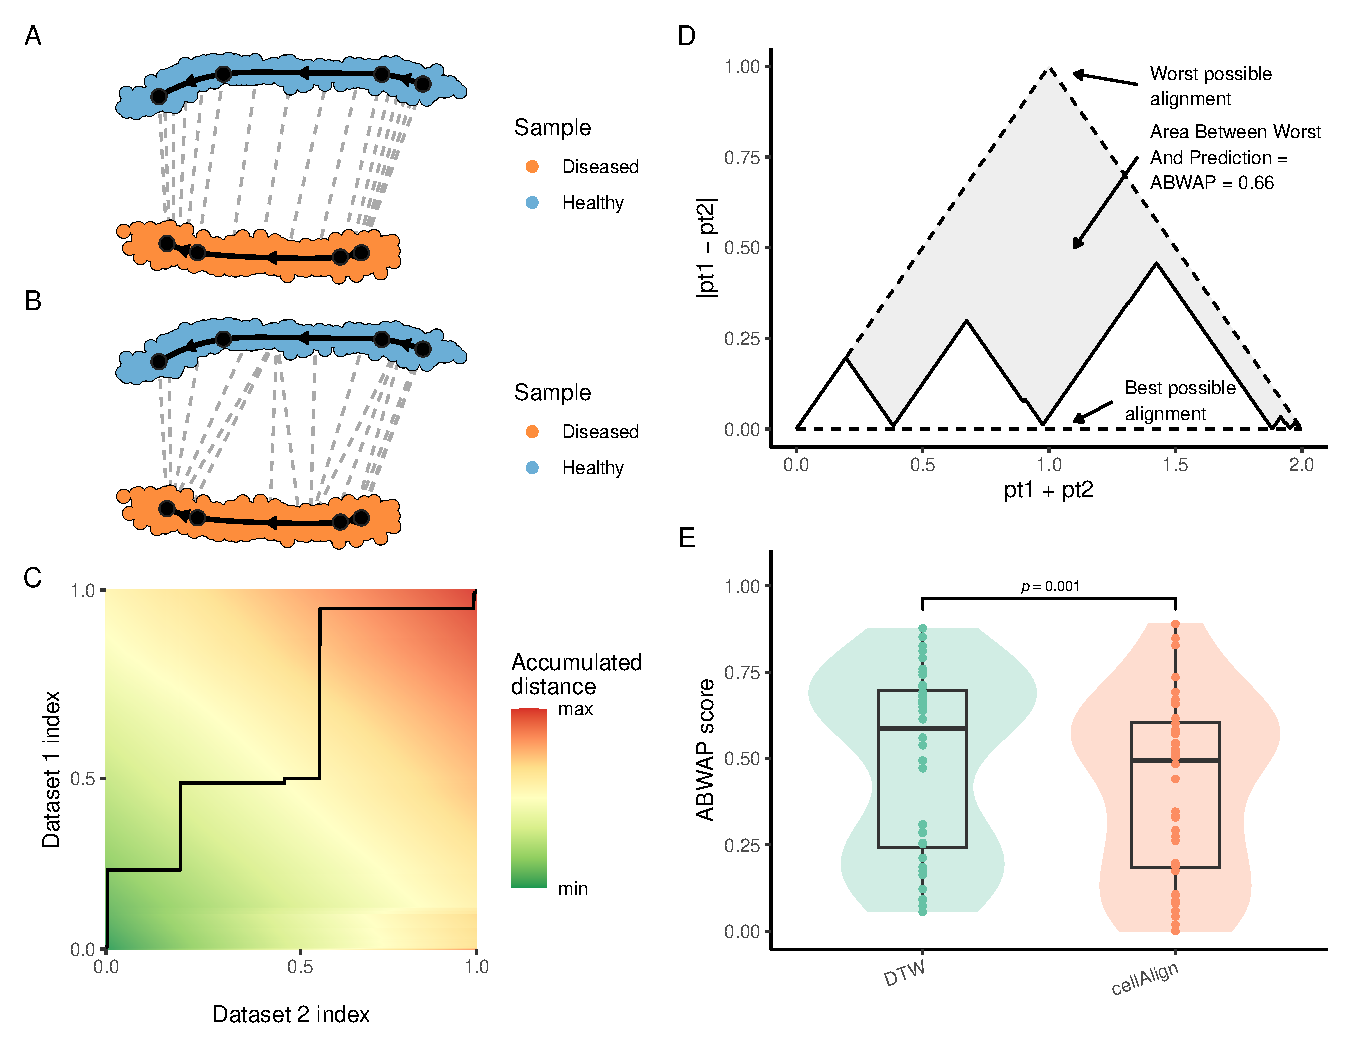
\includegraphics[width=\linewidth]{result_files/usecase_trajectory_alignment/supp_fig.pdf}
    \caption{
            \textbf{dyngen allows benchmarking of trajectory alignment methods.} 
 \DIFdelbeginFL \textbf{\DIFdelFL{A, B}}%DIFAUXCMD
\DIFdelendFL \DIFaddbeginFL \textbf{\DIFaddFL{A}}\DIFaddendFL : \DIFdelbeginFL \DIFdelFL{Two samples containing a }\DIFdelendFL \DIFaddbeginFL \DIFaddFL{An example }\DIFaddendFL linear \DIFaddbeginFL \DIFaddFL{dataset in need of }\DIFaddendFL trajectory \DIFdelbeginFL \DIFdelFL{, generated by dyngen}\DIFdelendFL \DIFaddbeginFL \DIFaddFL{alignment}\DIFaddendFL . \DIFdelbeginFL \textbf{\DIFdelFL{C, D}}%DIFAUXCMD
\DIFdelendFL \DIFaddbeginFL \DIFaddFL{Dashed lines represent the gold-standard alignment between the two trajectories according to the respective pseudotimes.
  }\textbf{\DIFaddFL{B}}\DIFaddendFL : Result of the DTW alignment on the \DIFdelbeginFL \DIFdelFL{samples in }\textbf{\DIFdelFL{A}} %DIFAUXCMD
\DIFdelFL{and }\textbf{\DIFdelFL{B}}%DIFAUXCMD
\DIFdelendFL \DIFaddbeginFL \DIFaddFL{two trajectories}\DIFaddendFL . 
 \DIFdelbeginFL \DIFdelFL{In }\DIFdelendFL \textbf{C}\DIFdelbeginFL \DIFdelFL{, the individual mappings of the alignment between cells are shown. In }\textbf{\DIFdelFL{D}}%DIFAUXCMD
\DIFdelFL{, the }\DIFdelendFL \DIFaddbeginFL \DIFaddFL{: DTW calculates an }\DIFaddendFL accumulated distance matrix\DIFdelbeginFL \DIFdelFL{between the two trajectories is shown}\DIFdelendFL \DIFaddbeginFL \DIFaddFL{. In this matrix}\DIFaddendFL , \DIFdelbeginFL \DIFdelFL{including the black }\DIFdelendFL \DIFaddbeginFL \DIFaddFL{a }\DIFaddendFL warping path \DIFaddbeginFL \DIFaddFL{(shown in black)}\DIFaddendFL , \DIFdelbeginFL \DIFdelFL{corresponding to these cell to cell alignments }\DIFdelendFL \DIFaddbeginFL \DIFaddFL{following a valley }\DIFaddendFL in \DIFdelbeginFL \textbf{\DIFdelFL{C}}%DIFAUXCMD
\DIFdelendFL \DIFaddbeginFL \DIFaddFL{the matrix from the bottom left to the top right corner is found}\DIFaddendFL . \DIFdelbeginFL \textbf{\DIFdelFL{E, F}}%DIFAUXCMD
\DIFdelFL{: Shows }\DIFdelendFL \DIFaddbeginFL \DIFaddFL{This shows how }\DIFaddendFL the \DIFdelbeginFL \DIFdelFL{accumulated distance matrices obtained after using DTW on two }\DIFdelendFL trajectories \DIFdelbeginFL \DIFdelFL{where noise (noise level }\DIFdelendFL \DIFaddbeginFL \DIFaddFL{best match each other.
  }\textbf{\DIFaddFL{D}}\DIFaddFL{: Illustration }\DIFaddendFL of \DIFdelbeginFL \DIFdelFL{0.4}\DIFdelendFL \DIFaddbeginFL \DIFaddFL{the Area Between Worst and Prediction (ABWAP}\DIFaddendFL ) \DIFdelbeginFL \DIFdelFL{was added }\DIFdelendFL \DIFaddbeginFL \DIFaddFL{metric. The warping path from subfigure C is mapped }\DIFaddendFL to the \DIFdelbeginFL \DIFdelFL{count matrix}\DIFdelendFL \DIFaddbeginFL \DIFaddFL{respective pseudotimes from both trajectories}\DIFaddendFL . \DIFdelbeginFL \DIFdelFL{In E the complete count matrices were used }\DIFdelendFL \DIFaddbeginFL \DIFaddFL{The ABWAP score is equal }\DIFaddendFL to \DIFdelbeginFL \DIFdelFL{perform }\DIFdelendFL the \DIFdelbeginFL \DIFdelFL{alignment. In F, smoothed pseudocells were used.
  }\textbf{\DIFdelFL{G:}} %DIFAUXCMD
\DIFdelFL{Shows }\DIFdelendFL \DIFaddbeginFL \DIFaddFL{area between }\DIFaddendFL the \DIFdelbeginFL \DIFdelFL{influence of added noise to }\DIFdelendFL \DIFaddbeginFL \DIFaddFL{prediction and }\DIFaddendFL the \DIFdelbeginFL \DIFdelFL{different processing methods}\DIFdelendFL \DIFaddbeginFL \DIFaddFL{worst possible prediction}\DIFaddendFL . 
  \DIFdelbeginFL \DIFdelFL{We can see that }\DIFdelendFL \DIFaddbeginFL \textbf{\DIFaddFL{E:}} \DIFaddFL{An evaluation of }\DIFaddendFL DTW \DIFdelbeginFL \DIFdelFL{+ smoothing performs best }\DIFdelendFL \DIFaddbeginFL \DIFaddFL{versus cellAlign on 40 different linear trajectories, }\DIFaddendFL in \DIFdelbeginFL \DIFdelFL{noisy circumstances}\DIFdelendFL \DIFaddbeginFL \DIFaddFL{which cellAlign significantly outperforms DTW}\DIFaddendFL .
    }
    \label{fig:traj_align}
\end{figure}

\begin{figure}[H]
    \centering
    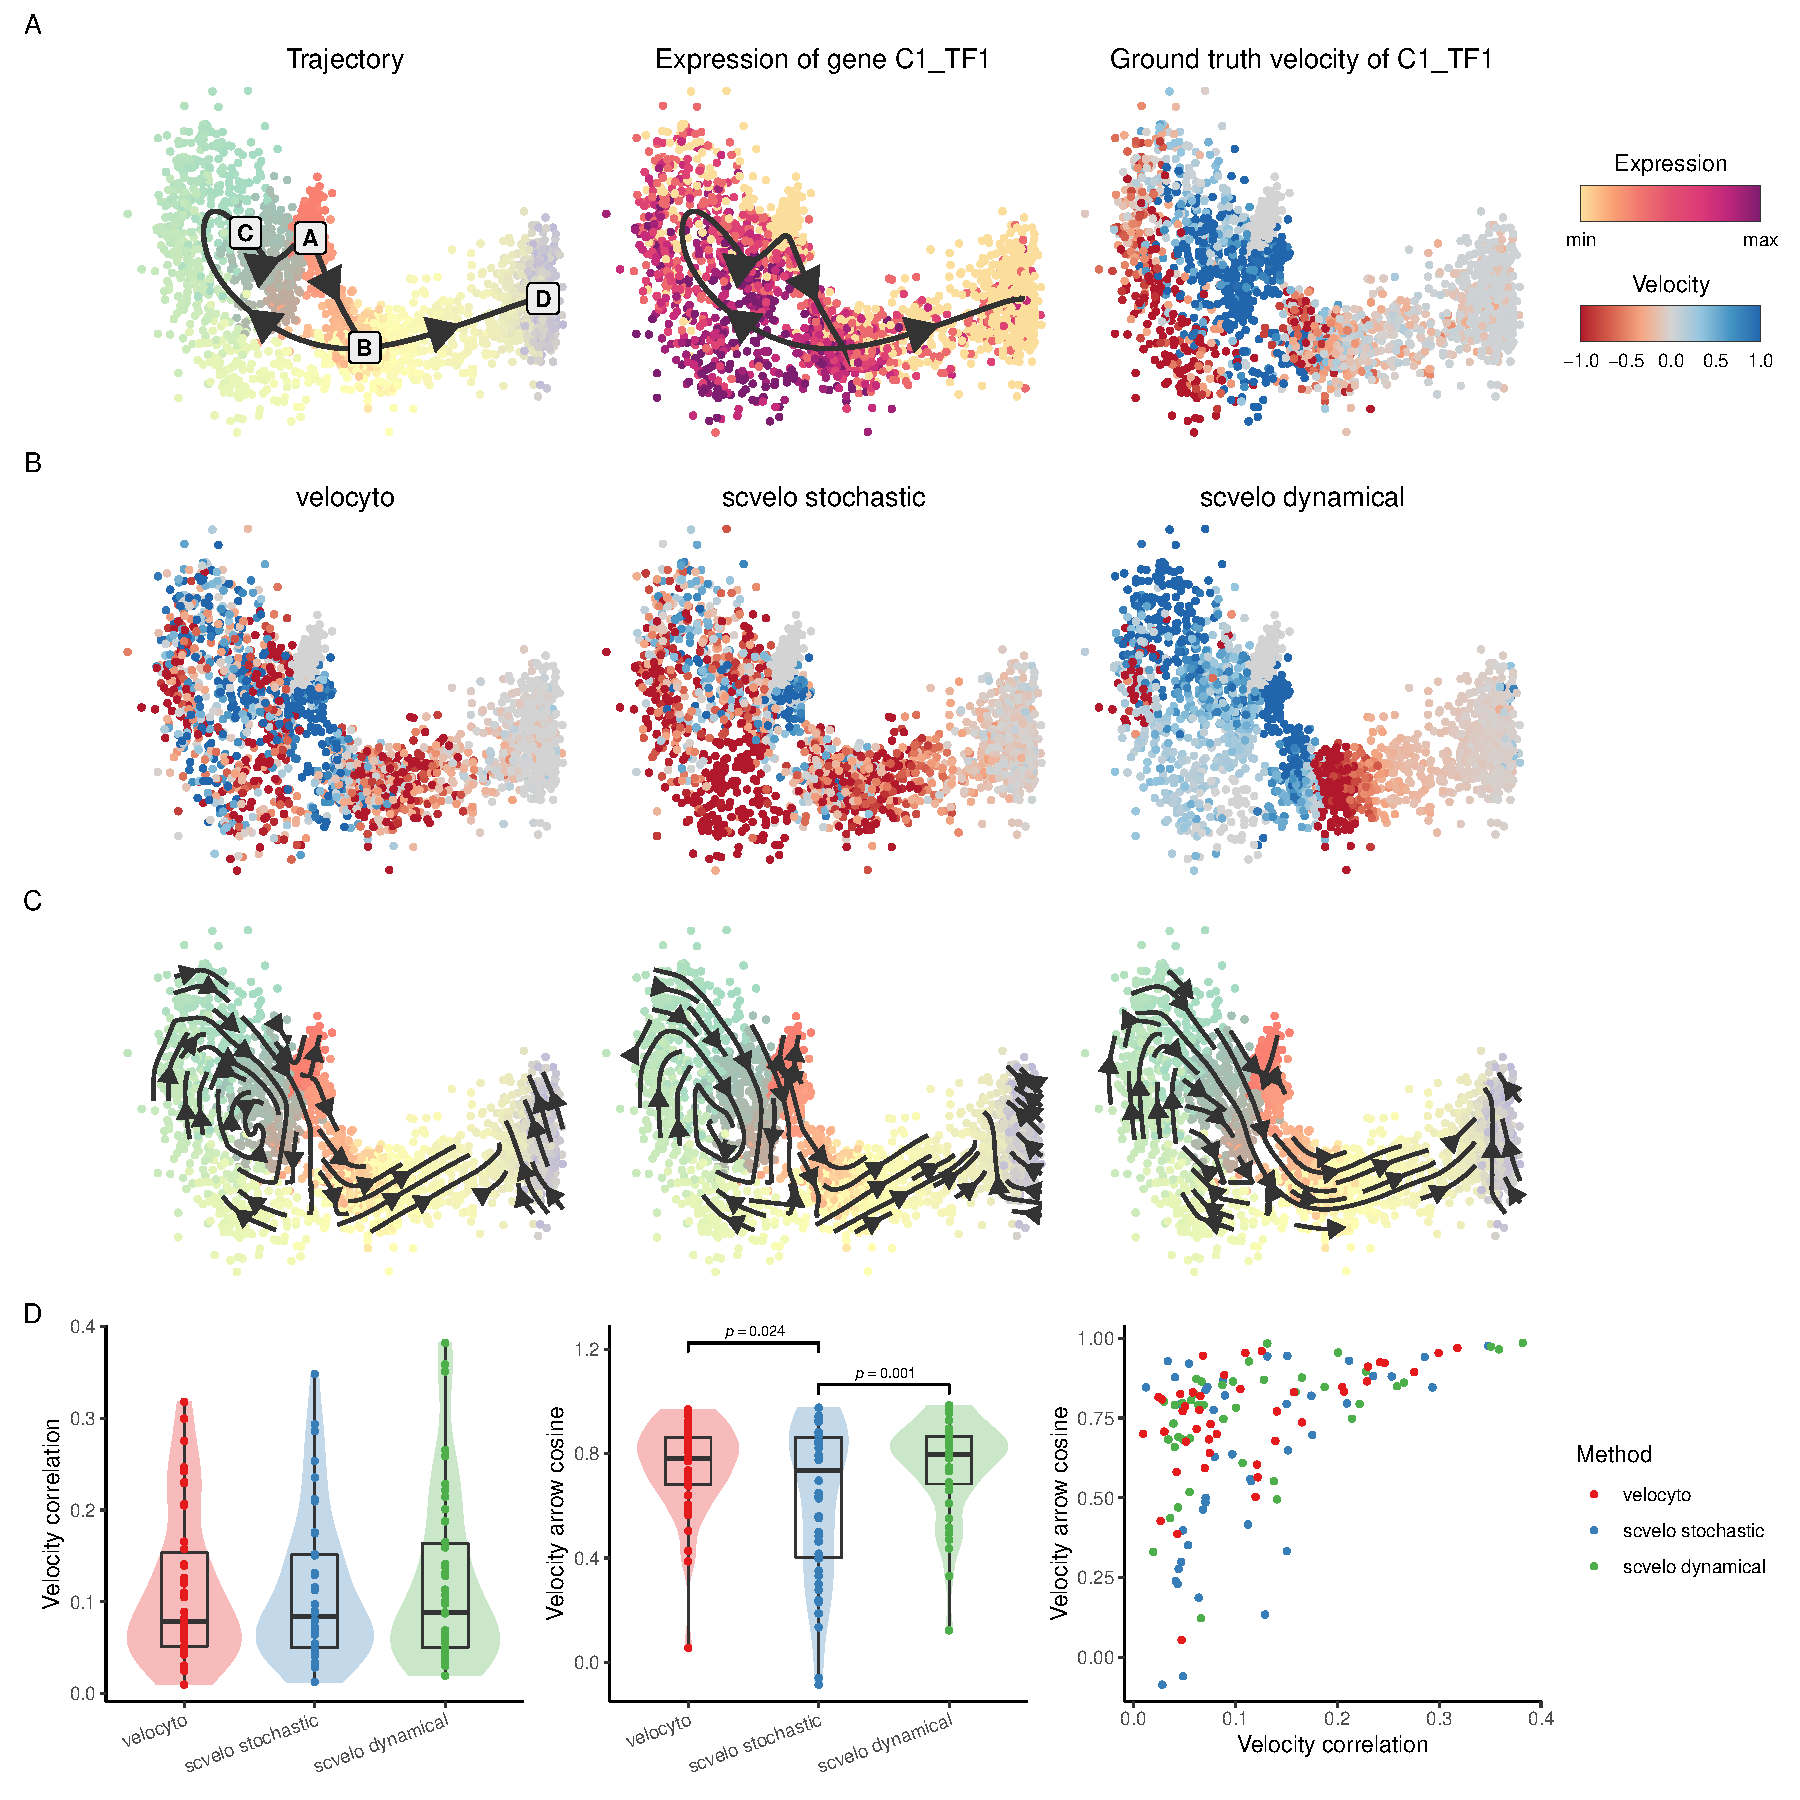
\includegraphics[width=\linewidth]{result_files/usecase_rna_velocity/supp_fig.pdf}
    \caption{
            \textbf{dyngen allows benchmarking of RNA velocity methods.} 
            \textbf{A:} \DIFdelbeginFL \DIFdelFL{An example }\DIFdelendFL \DIFaddbeginFL \DIFaddFL{The ground-truth information of a }\DIFaddendFL bifurcating \DIFdelbeginFL \DIFdelFL{cycle }\DIFdelendFL dataset\DIFaddbeginFL \DIFaddFL{: ground-truth trajectory (left)}\DIFaddendFL , \DIFdelbeginFL \DIFdelFL{with as illustration the }\DIFdelendFL \DIFaddbeginFL \DIFaddFL{gene }\DIFaddendFL expression \DIFdelbeginFL \DIFdelFL{and ground truth velocity }\DIFdelendFL of a gene \DIFdelbeginFL \DIFdelFL{D1}\DIFdelendFL \DIFaddbeginFL \DIFaddFL{B5}\DIFaddendFL \_TF1 \DIFdelbeginFL \DIFdelFL{that goes up }\DIFdelendFL \DIFaddbeginFL \DIFaddFL{(middle), }\DIFaddendFL and \DIFdelbeginFL \DIFdelFL{down in one branch of }\DIFdelendFL the \DIFdelbeginFL \DIFdelFL{trajectory}\DIFdelendFL \DIFaddbeginFL \DIFaddFL{RNA velocity of B5\_TF1 (right)}\DIFaddendFL .
\textbf{B:} The RNA velocity estimates of gene \DIFdelbeginFL \DIFdelFL{D1}\DIFdelendFL \DIFaddbeginFL \DIFaddFL{B5}\DIFaddendFL \_TF1 by the different methods.
\textbf{C:} The velocity stream plots produced from the predictions of each method, as generated by scvelo.
\textbf{D:} The predictions scored by two different metrics, the velocity correlation and the velocity arrow cosine. The velocity correlation is the correlation between the ground-truth velocity (A, right) and the predicted velocity (B). The velocity arrow cosine is the cosine similarity between the direction of segments of the ground-truth trajectory (A, left) and the RNA velocity values calculated at those points (C). 
    }
    \label{fig:velocity}
\end{figure}

\begin{figure}[H]
    \centering
    \DIFdelbeginFL %DIFDELCMD < 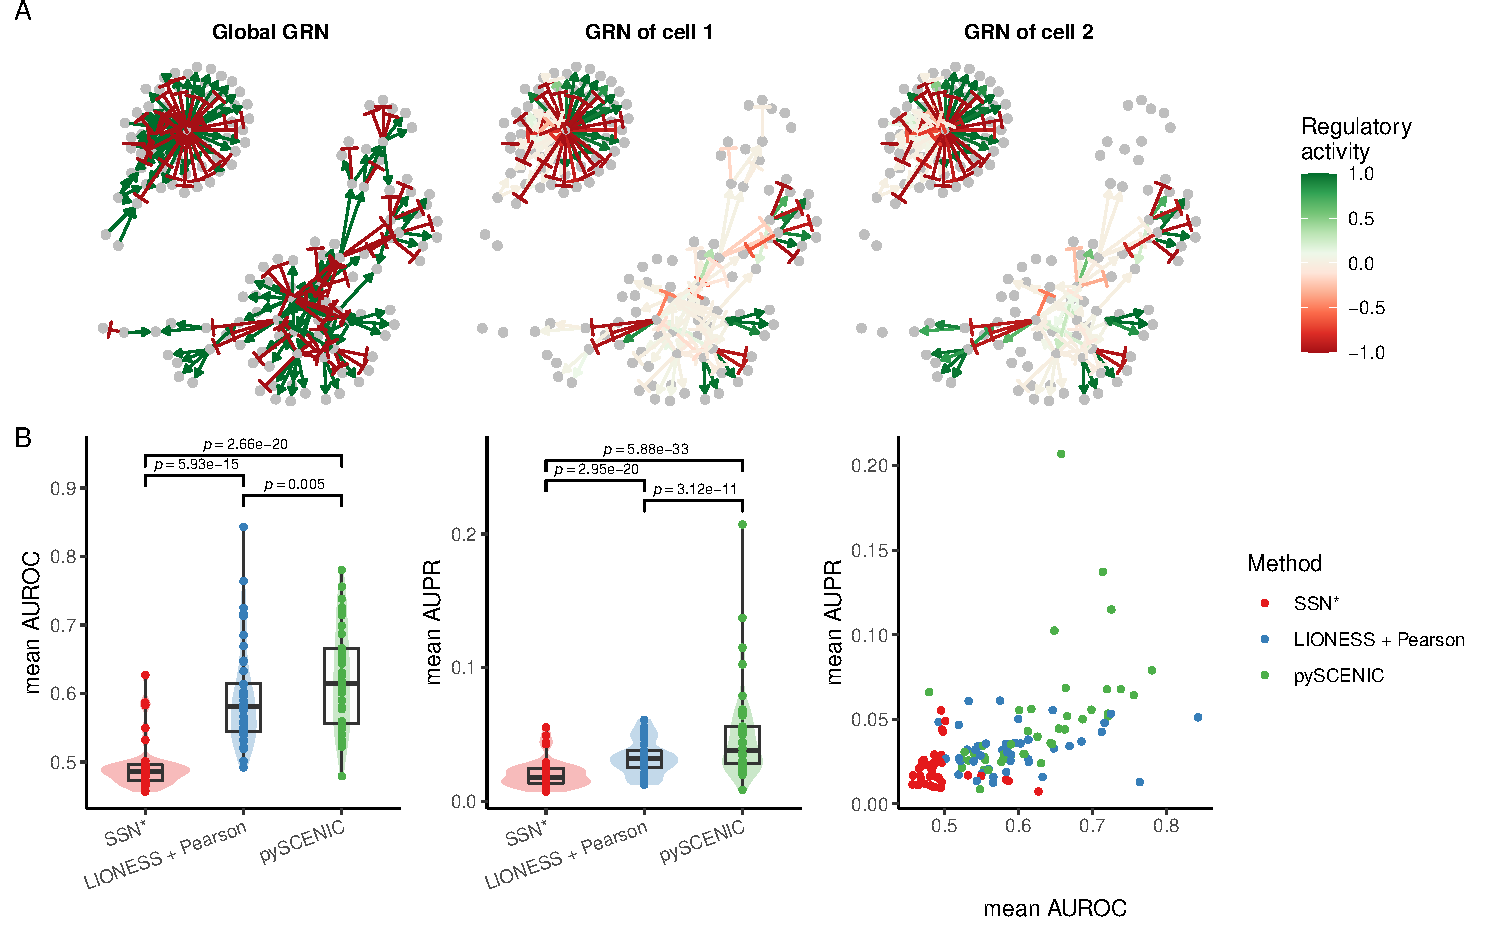
\includegraphics[width=.8\linewidth]{result_files/usecase_network_inference/supp_fig.pdf}
%DIFDELCMD <     %%%
\DIFdelendFL \DIFaddbeginFL 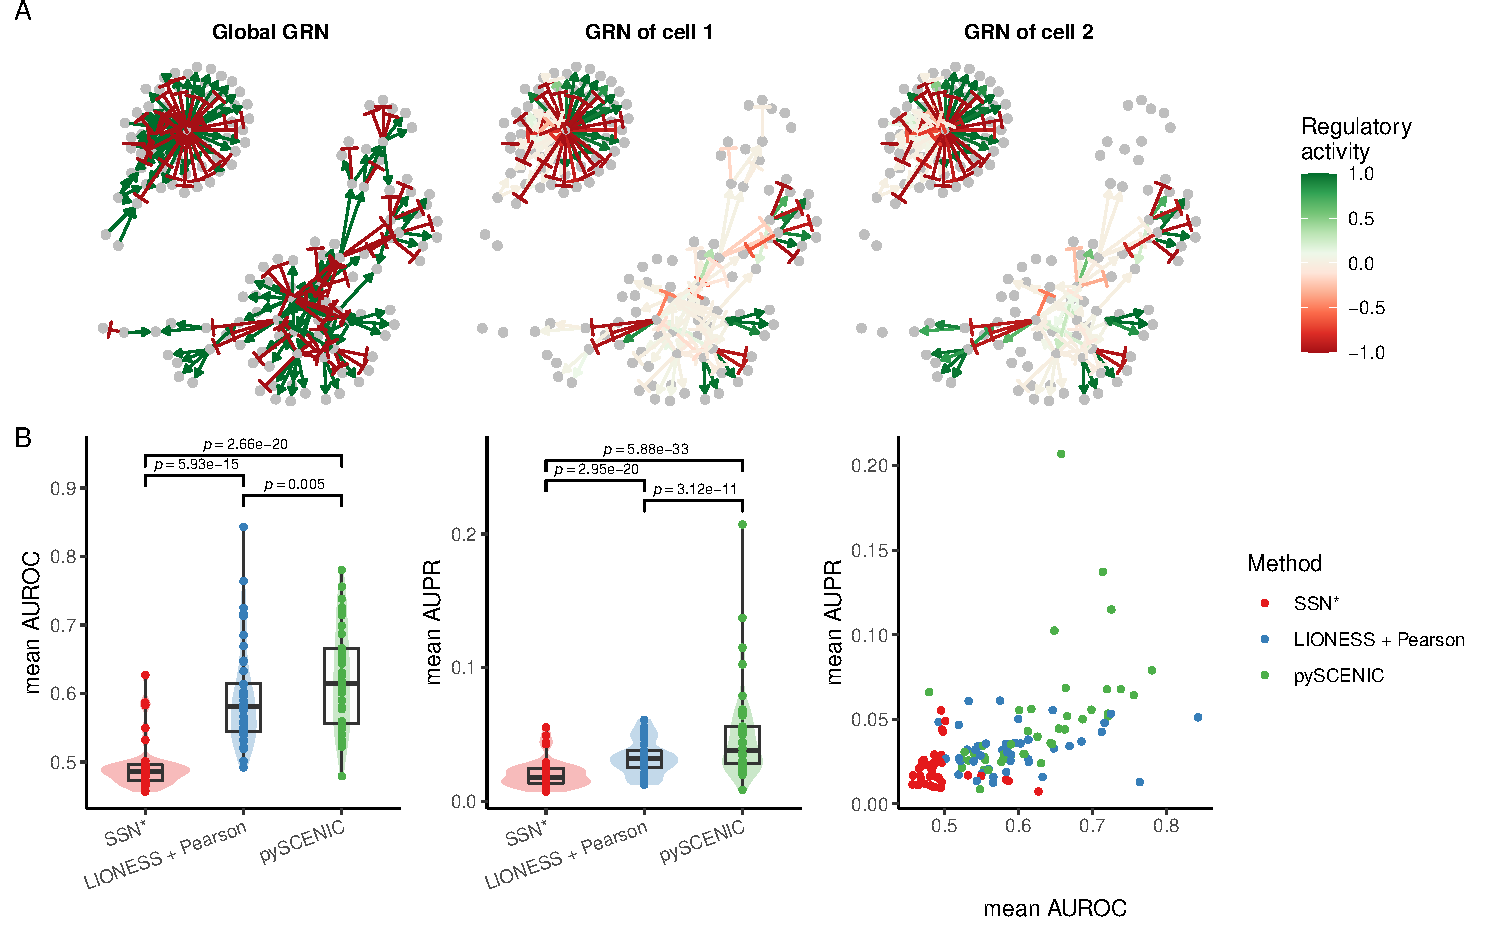
\includegraphics[width=\linewidth]{result_files/usecase_network_inference/supp_fig.pdf}
    \DIFaddendFL \caption{
            \textbf{dyngen allows benchmarking Cell-specific Network Inference (CSNI) methods.} 
            \textbf{A:} A cell is simulated using the global gene regulatory network (GRN, top left). However, at any particular state in the simulation, only a fraction of the gene regulatory interactions are active.
            \textbf{B:} CSNI methods were executed to predict the regulatory interactions that are active in each cell specifically. Using the ground-truth cell-specific GRN, the performance of each method was quantified on \DIFdelbeginFL \DIFdelFL{14 }\DIFdelendFL \DIFaddbeginFL \DIFaddFL{42 }\DIFaddendFL dyngen datasets. 
    }
    \label{fig:scgrn}
\end{figure}

\begin{figure}[H]
    \centering
    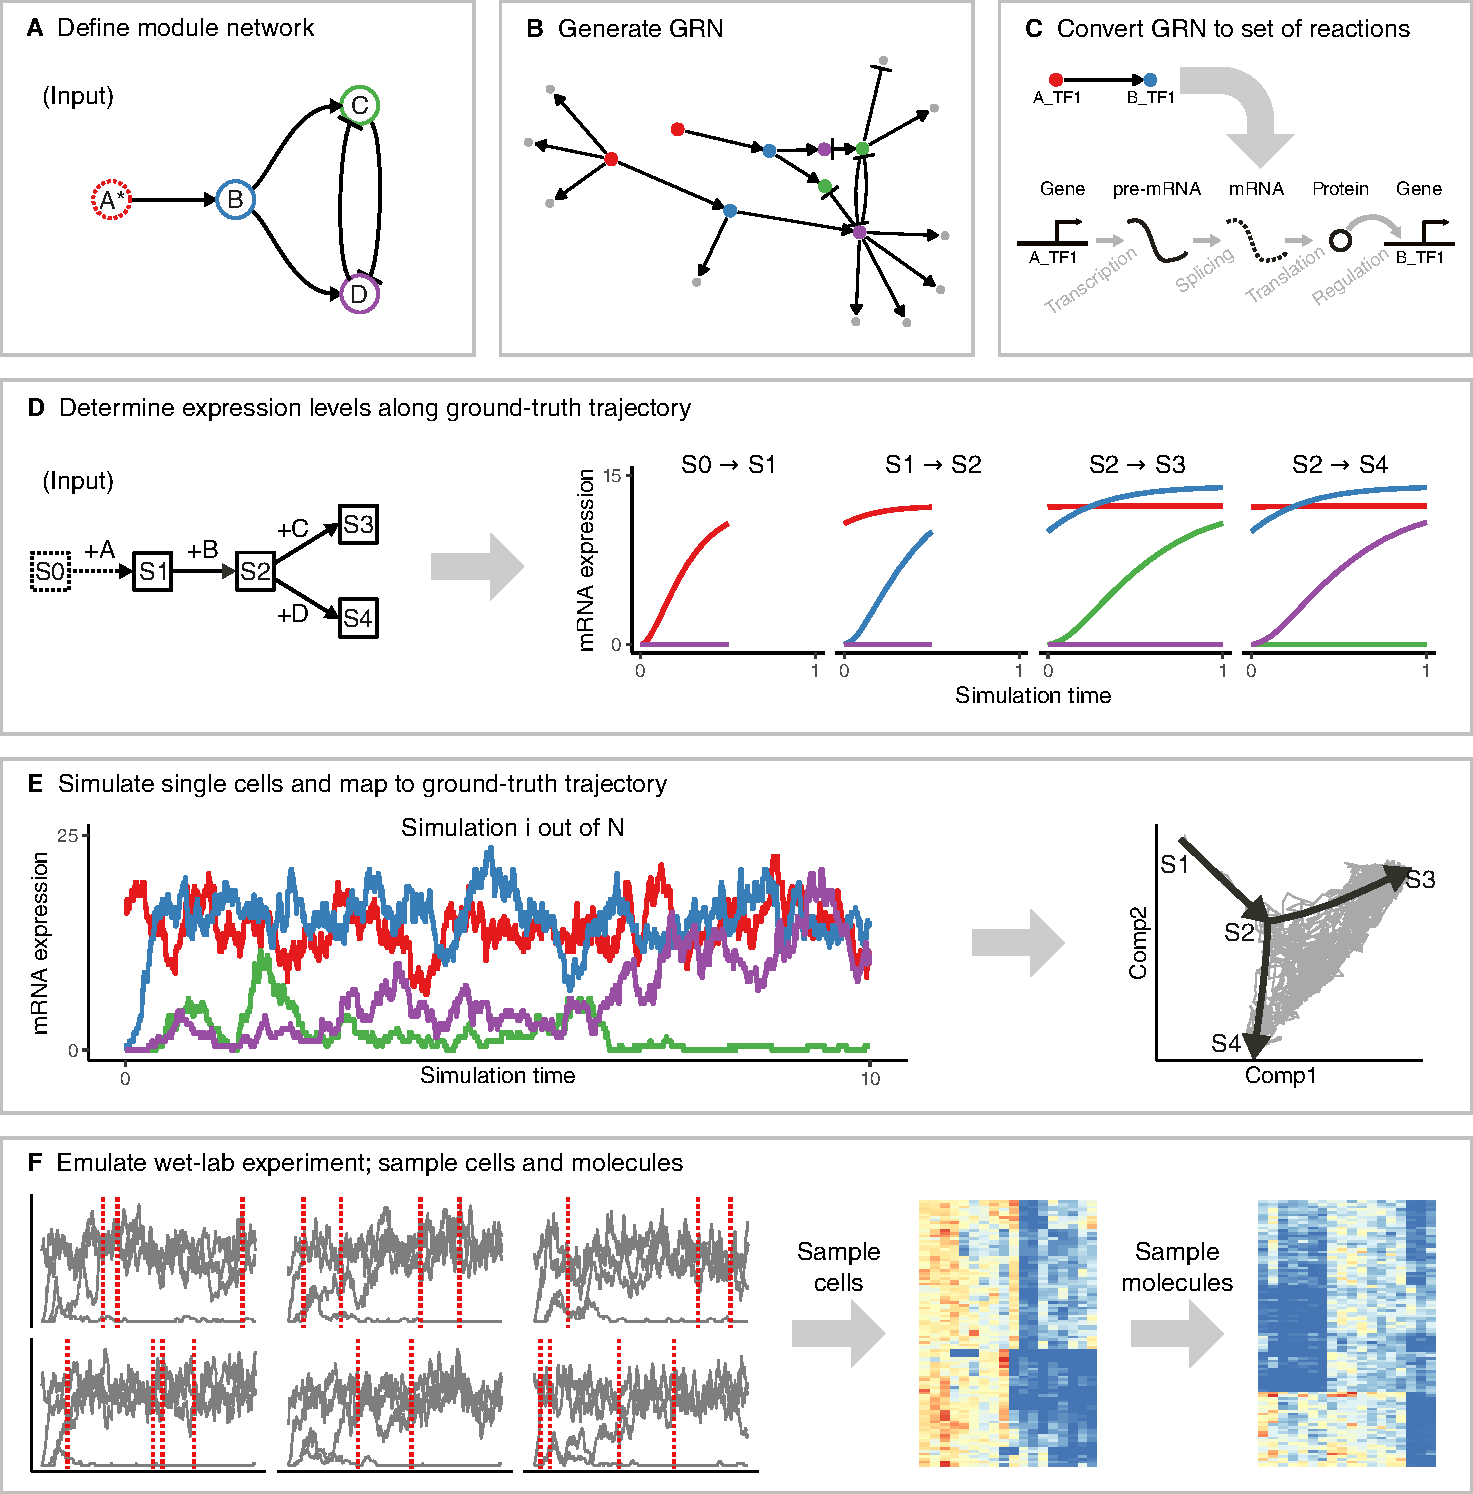
\includegraphics[width=\textwidth]{result_files/explain_methods}
    \caption{\textbf{The workflow of dyngen consists of six main steps.} 
    \textbf{A:} The user needs to specify the desired module network or use a predefined module network. The module network is what determines the dynamic behaviour of simulated cells.
    \textbf{B:} The number of desired transcription factors (which drive the desired dynamic process) are amongst the given modules and adds regulatory interactions according to the module network. Additional target genes (which do not influence the dynamic process) are added by sampling interactions from GRN interaction databases.
    \textbf{C:} Each gene regulatory interaction in the GRN is converted to a set of biochemical reactions. 
    \textbf{D:} Along with the module network, the user also needs to specify the backbone structure of expected cell states. The average expression of each edge in the backbone is simulated by activating a restricted set of genes for each edge. 
    \textbf{E:} Multiple Gillespie SSA simulations are run using the reactions defined in step C.  The counts of each of the molecules at each time step are extracted. Each time step is mapped to a point in the backbone. 
    \textbf{F:} The molecule levels of multiple simulations are shown over time (left). From each simulation, multiple cells are sampled (from left to middle). Technical noise from profiling is simulated by sampling molecules from the set of molecules inside each cell (from middle to right).
    }
    \label{fig:explain_methods}
\end{figure}

\begin{figure}[H]
    \centering
    \includegraphics[width=0.8\textwidth]{result_files/example_backbones_onlymodules}
    \caption{
      \textbf{The module network determines the type of dynamic process which simulated cells will undergo.} A module network describes the regulatory interactions between sets of transcription factors which drive the desired dynamic process.
    }
    \label{fig:example_backbones_onlymodules}
\end{figure}

\begin{figure}[H]
    \centering
    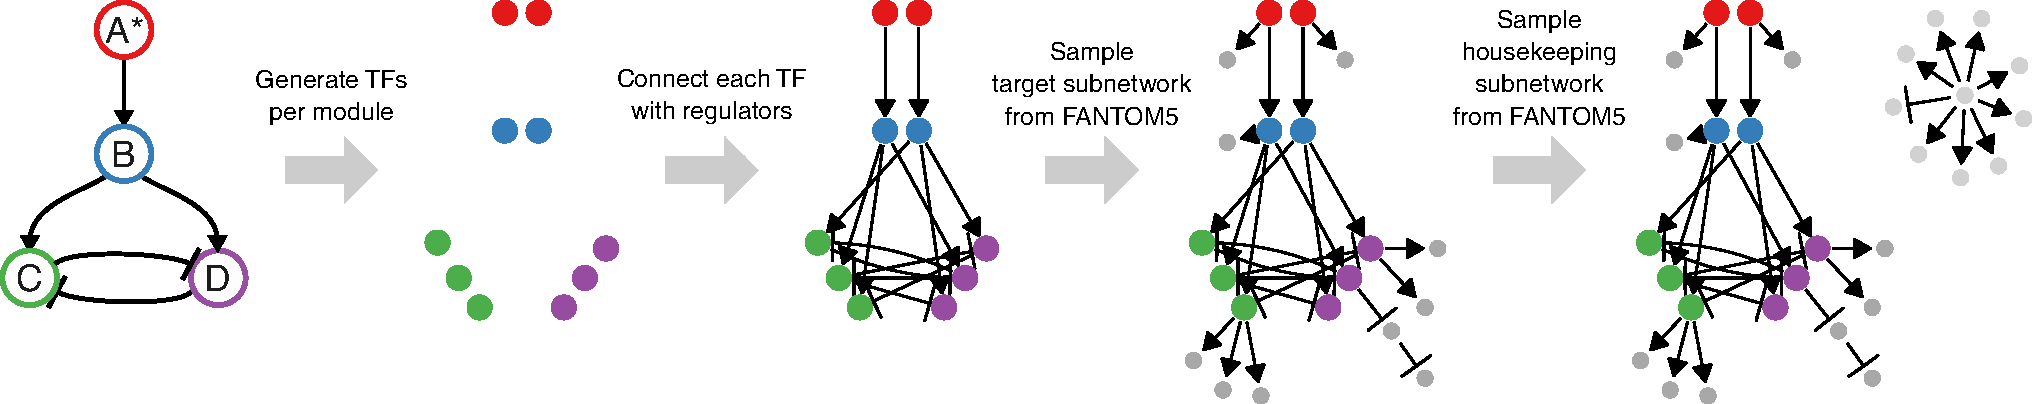
\includegraphics[width=\linewidth]{result_files/gen_feature_network}
    \caption{
        \textbf{Generating the feature network from a backbone consists of four main steps.}
    }
    \label{fig:gen_feature_network}
\end{figure}

\begin{table}[H]
    \caption{
      \textbf{Reactions affecting the abundance levels of pre-mRNA $\text{x}_{G}$, mature mRNA $\text{y}_{G}$ and proteins $\text{z}_{G}$ of gene $G$.} Define the set of regulators of $G$ as $\text{R}_{G}$, the set of upregulating regulators of $G$ as $\text{R}^+_{G}$, and the set of down-regulating regulators of $G$ as $\text{R}^-_{G}$. Parameters used in the propensity formulae are defined in Table \ref{tab:reaction_params}.
    } \label{tab:reaction_def}
    \centering
    \begin{tabular}{|lcc|}
        \hline
        Reaction & Effect & Propensity \\ \hline \hline
        Transcription & $\emptyset \rightarrow \text{x}_{G}$ & $\text{xpr}_{G} \times \frac{\text{bas}_{G} - \text{ind}_{G}^{|\text{R}^+_{G}|} + \prod\limits_{H \in \text{R}^+_{G}}(\text{ind}_{G} + \text{bind}_{G,H})}{\prod\limits_{H \in \text{R}_{G}}(1 + \text{bind}_{G,H})}$ \\
        Splicing & $\text{x}_{G} \rightarrow \text{y}_{G}$ & $\text{ysr}_{G} \times \text{x}_{G}$ \\
        Translation & $\text{y}_{G} \rightarrow \text{y}_{G} + \text{z}_{G}$ & $\text{zpr}_{G} \times \text{y}_{G}$ \\ \hline\hline
        Pre-mRNA degradation & $\text{x}_{G} \rightarrow \emptyset$ & $\text{ydr}_{G} \times \text{x}_{G}$ \\
        Mature mRNA degradation & $\text{y}_{G} \rightarrow \emptyset$ & $\text{ydr}_{G} \times \text{y}_{G}$ \\
        Protein degradation & $\text{z}_{G} \rightarrow \emptyset$ & $\text{zdr}_{G} \times \text{z}_{G}$ \\ \hline
    \end{tabular}
\end{table}

\begin{table}[H]
    \caption{
      \textbf{Default parameters defined for the calculation of reaction propensity functions.}
    } \label{tab:reaction_params}
    \centering
    \begin{tabular}{|lrl|}
        \hline
        Parameter & Symbol & Definition \\ \hline \hline
        Transcription rate & $\text{xpr}_{G}$ & $\in U(10, 20)$ \\
        Splicing rate & $\text{ysr}_{G}$ & $= \ln(2)\ /\ 2$ \\
        Translation rate & $\text{zpr}_{G}$ & $\in U(100, 150)$ \\
        (Pre-)mRNA half-life & $\text{yhl}_{G}$ & $\in U(2.5, 5)$ \\
        Protein half-life & $\text{zhl}_{G}$ & $\in U(5, 10)$ \\
        Interaction strength & $\text{str}_{G,H}$ & $\in 10^{U(0, 2)}$ * \\
        Hill coefficient & $\text{hill}_{G,H}$ & $\in U(0.5, 2)$ * \\
        Independence factor & $\text{ind}_{G}$ & $\in U(0, 1)$ * \\ \hline\hline
        (Pre-)mRNA degradation rate & $\text{ydr}_{G}$ & $= \ln(2)\ /\ \text{yhl}_{G}$ \\
        Protein degradation rate & $\text{zdr}_{G}$ & $= \ln(2)\ /\ \text{zhl}_{G}$ \\
        Dissociation constant & $\text{dis}_{H}$ & $= 0.5 \times \frac{\text{xpr}_{H} \times \text{ysr}_{H} \times \text{zpr}_{H}}{(\text{ydr}_{H} + \text{ysr}_{H}) \times \text{ydr}_{H} \times \text{zdr}_{H}}$ \\
        Binding strength & $\text{bind}_{G,H}$ & $= \text{str}_{G,H} \times \left(\text{z}_{H}\ /\ \text{dis}_{H}\right) ^ {\text{hill}_{G,H}}$ \\
        Basal expression & $\text{bas}_{G}$ & $= \begin{cases} 1 & \mbox{if } \text{R}^+_{G} = \emptyset \\ 0.0001 & \mbox{if } \text{R}^-_{G} = \emptyset \mbox{ and } \text{R}^+_{G} \neq \emptyset \\ 0.5 & \mbox{otherwise} \end{cases}$ * \\ \hline
        \multicolumn{3}{l}{*: unless $G$ is a TF, then the value is determined by the backbone.}
    \end{tabular}
\end{table}

\begin{figure}[H]
    \centering
    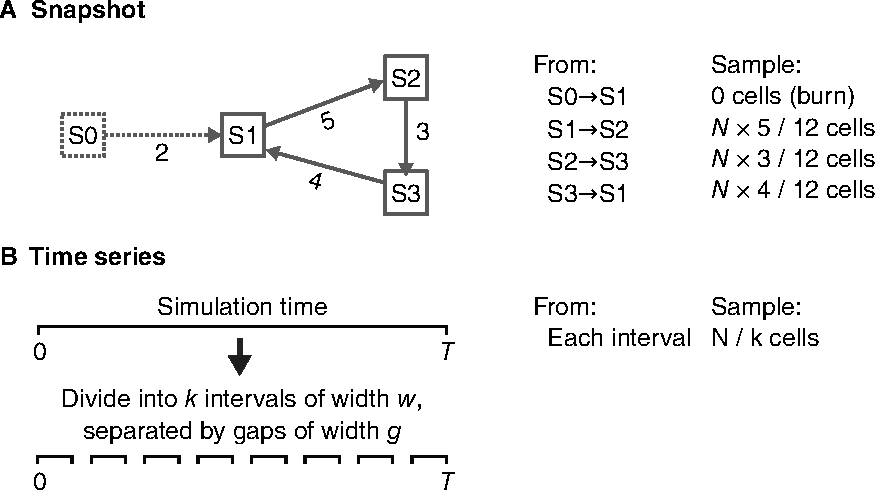
\includegraphics[width=.6\linewidth]{result_files/sample_cells.pdf}
    \caption{
        \textbf{Two approaches can be used to sample cells from simulations: snapshot and time-series.}
    }
    \label{fig:sample_cells}
\end{figure}

\begin{figure}[H]
    \centering
    \includegraphics[width=0.8\textwidth]{result_files/example_backbones}
    \caption{\textbf{Examples of the ground-truth state networks which need to be provided alongside the module network.}}
    \label{fig:example_backbones}
\end{figure}

\printbibliography

\end{document}
